\documentclass[twoside]{book}

% Packages required by doxygen
\usepackage{fixltx2e}
\usepackage{calc}
\usepackage{doxygen}
\usepackage[export]{adjustbox} % also loads graphicx
\usepackage{graphicx}
\usepackage[utf8]{inputenc}
\usepackage{makeidx}
\usepackage{multicol}
\usepackage{multirow}
\PassOptionsToPackage{warn}{textcomp}
\usepackage{textcomp}
\usepackage[nointegrals]{wasysym}
\usepackage[table]{xcolor}

% Font selection
\usepackage[T1]{fontenc}
\usepackage[scaled=.90]{helvet}
\usepackage{courier}
\usepackage{amssymb}
\usepackage{sectsty}
\renewcommand{\familydefault}{\sfdefault}
\allsectionsfont{%
  \fontseries{bc}\selectfont%
  \color{darkgray}%
}
\renewcommand{\DoxyLabelFont}{%
  \fontseries{bc}\selectfont%
  \color{darkgray}%
}
\newcommand{\+}{\discretionary{\mbox{\scriptsize$\hookleftarrow$}}{}{}}

% Page & text layout
\usepackage{geometry}
\geometry{%
  a4paper,%
  top=2.5cm,%
  bottom=2.5cm,%
  left=2.5cm,%
  right=2.5cm%
}
\tolerance=750
\hfuzz=15pt
\hbadness=750
\setlength{\emergencystretch}{15pt}
\setlength{\parindent}{0cm}
\setlength{\parskip}{3ex plus 2ex minus 2ex}
\makeatletter
\renewcommand{\paragraph}{%
  \@startsection{paragraph}{4}{0ex}{-1.0ex}{1.0ex}{%
    \normalfont\normalsize\bfseries\SS@parafont%
  }%
}
\renewcommand{\subparagraph}{%
  \@startsection{subparagraph}{5}{0ex}{-1.0ex}{1.0ex}{%
    \normalfont\normalsize\bfseries\SS@subparafont%
  }%
}
\makeatother

% Headers & footers
\usepackage{fancyhdr}
\pagestyle{fancyplain}
\fancyhead[LE]{\fancyplain{}{\bfseries\thepage}}
\fancyhead[CE]{\fancyplain{}{}}
\fancyhead[RE]{\fancyplain{}{\bfseries\leftmark}}
\fancyhead[LO]{\fancyplain{}{\bfseries\rightmark}}
\fancyhead[CO]{\fancyplain{}{}}
\fancyhead[RO]{\fancyplain{}{\bfseries\thepage}}
\fancyfoot[LE]{\fancyplain{}{}}
\fancyfoot[CE]{\fancyplain{}{}}
\fancyfoot[RE]{\fancyplain{}{\bfseries\scriptsize Generated by Doxygen }}
\fancyfoot[LO]{\fancyplain{}{\bfseries\scriptsize Generated by Doxygen }}
\fancyfoot[CO]{\fancyplain{}{}}
\fancyfoot[RO]{\fancyplain{}{}}
\renewcommand{\footrulewidth}{0.4pt}
\renewcommand{\chaptermark}[1]{%
  \markboth{#1}{}%
}
\renewcommand{\sectionmark}[1]{%
  \markright{\thesection\ #1}%
}

% Indices & bibliography
\usepackage{natbib}
\usepackage[titles]{tocloft}
\setcounter{tocdepth}{3}
\setcounter{secnumdepth}{5}
\makeindex

% Hyperlinks (required, but should be loaded last)
\usepackage{ifpdf}
\ifpdf
  \usepackage[pdftex,pagebackref=true]{hyperref}
\else
  \usepackage[ps2pdf,pagebackref=true]{hyperref}
\fi
\hypersetup{%
  colorlinks=true,%
  linkcolor=blue,%
  citecolor=blue,%
  unicode%
}

% Custom commands
\newcommand{\clearemptydoublepage}{%
  \newpage{\pagestyle{empty}\cleardoublepage}%
}

\usepackage{caption}
\captionsetup{labelsep=space,justification=centering,font={bf},singlelinecheck=off,skip=4pt,position=top}

%===== C O N T E N T S =====

\begin{document}

% Titlepage & ToC
\hypersetup{pageanchor=false,
             bookmarksnumbered=true,
             pdfencoding=unicode
            }
\pagenumbering{roman}
\begin{titlepage}
\vspace*{7cm}
\begin{center}%
{\Large E\+F-\/\+M\+AP }\\
\vspace*{1cm}
{\large Generated by Doxygen 1.8.11}\\
\end{center}
\end{titlepage}
\clearemptydoublepage
\tableofcontents
\clearemptydoublepage
\pagenumbering{arabic}
\hypersetup{pageanchor=true}

%--- Begin generated contents ---
\chapter{Accueil}
\label{index}\hypertarget{index}{}\hypertarget{index_intro_sec}{}\section{Introduction}\label{index_intro_sec}
L\textquotesingle{}objectif de ce projet est la réalisation d\textquotesingle{}un solveur de problème de type E\+DP linéaires. Plus particulièrement, l\textquotesingle{}objectif principal est la résolution du problème dit du Micro-\/\+Onde, dont on fait ici le rappel de l\textquotesingle{}énoncé\+:\hypertarget{index_a}{}\subsection{Enoncé du problème}\label{index_a}
En version Helmholtz il s’agit de résoudre un probleme du type\+: Trouver u une fonction définie sur l’ouvert  a valeur dans C tel que

ω$^\wedge$2µu + ∇.1/ε∇u = 0 ∈ Ω avec des données aux bord imaginaires.

Le couplage avec la température θ, se fait comme suivant\+:

−∇.\+K∇θ = f

dans l’objet a cuire, et où f est nulle hors de l’objet a cuire, et est égal a uu dans l’objet a cuire.

Le projet est la résolution de 2 équations découples avec les données suivantes \+:

ε = 1 dans l’air et ε = 4 dans la viande.

On pourra prendre des conditions de Dirichlet sur l’objet a cuire.\hypertarget{index_Problématiques}{}\subsection{Problématiques}\label{index_Problématiques}
En étudiant l\textquotesingle{}énoncé ,on constate que ce projet comporte plusieurs points importants, liés à dés problématiques variées sur le plan de l\textquotesingle{}analyse numérique, de l\textquotesingle{}analyse matricielle ou encore de l\textquotesingle{}informatique.


\begin{DoxyItemize}
\item Le problème est tridimensionnel, cela implique une croissance cubique de la taille des matrices par rapport à la dimension du problème. Cela implique que la résolution des systèmes linéaires ne peut se faire par le biais d\textquotesingle{}un algorithme de résolution directe (décompositions Q\+R/\+LU), on préviligiera donc des méthodes itératives.
\item Le problème est vectoriel, mais l\textquotesingle{}opérateur est unique, i.\+e. chaque résolution comporte 3 \char`\"{}seconds membres\char`\"{} correspondant chacuns à l\textquotesingle{}une des dimensions dans laquelle le problème est résolu.
\item La matrice correspondant au problème discrétisé n\textquotesingle{}est pas nécessairment définie, elle est en revanche symétrique. Cela implique un choix préférentiel pour la résolution du système \+: la méthode M\+I\+N\+Res
\item Quant à la gestion des données d\textquotesingle{}entrée/sortie, l\textquotesingle{}énoncé reste vague, mais implique que le programme doit être capable de gérer les partitions de maillages. 
\end{DoxyItemize}
\chapter{Namespace Index}
\section{Namespace List}
Here is a list of all documented namespaces with brief descriptions\+:\begin{DoxyCompactList}
\item\contentsline{section}{\hyperlink{namespacestd}{std} \\*Espace de nommage standard }{\pageref{namespacestd}}{}
\end{DoxyCompactList}

\chapter{Hierarchical Index}
\section{Class Hierarchy}
This inheritance list is sorted roughly, but not completely, alphabetically\+:\begin{DoxyCompactList}
\item \contentsline{section}{BC}{\pageref{class_b_c}}{}
\item \contentsline{section}{C3}{\pageref{class_c3}}{}
\item \contentsline{section}{Maillage3D}{\pageref{class_maillage3_d}}{}
\item \contentsline{section}{Mat\+Sparse\+C3}{\pageref{class_mat_sparse_c3}}{}
\item \contentsline{section}{Point}{\pageref{struct_point}}{}
\item Q\+Dialog\begin{DoxyCompactList}
\item \contentsline{section}{Parameters\+Dialog}{\pageref{class_parameters_dialog}}{}
\item \contentsline{section}{Viewer3D}{\pageref{class_viewer3_d}}{}
\end{DoxyCompactList}
\item Q\+Geometry\begin{DoxyCompactList}
\item \contentsline{section}{Triangle\+Mesh\+Geometry}{\pageref{class_triangle_mesh_geometry}}{}
\end{DoxyCompactList}
\item Q\+Geometry\+Renderer\begin{DoxyCompactList}
\item \contentsline{section}{Triangle\+Mesh\+Renderer}{\pageref{class_triangle_mesh_renderer}}{}
\end{DoxyCompactList}
\item Q\+Object\begin{DoxyCompactList}
\item \contentsline{section}{F\+E\+Problem}{\pageref{class_f_e_problem}}{}
\item \contentsline{section}{Orbit\+Transform\+Controller}{\pageref{class_orbit_transform_controller}}{}
\item \contentsline{section}{Scatter\+Data\+Modifier}{\pageref{class_scatter_data_modifier}}{}
\item \contentsline{section}{Scene\+Modifier}{\pageref{class_scene_modifier}}{}
\end{DoxyCompactList}
\item Q\+Widget\begin{DoxyCompactList}
\item \contentsline{section}{M\+A\+P\+\_\+\+Main\+Window}{\pageref{class_m_a_p___main_window}}{}
\item \contentsline{section}{Qt3\+D\+Widget}{\pageref{class_qt3_d_widget}}{}
\end{DoxyCompactList}
\item \contentsline{section}{R2}{\pageref{class_r2}}{}
\item \contentsline{section}{R3}{\pageref{class_r3}}{}
\item \contentsline{section}{R\+HS}{\pageref{class_r_h_s}}{}
\item \contentsline{section}{Solver}{\pageref{class_solver}}{}
\item \contentsline{section}{Triangle}{\pageref{struct_triangle}}{}
\item \contentsline{section}{util}{\pageref{classutil}}{}
\item \contentsline{section}{Vector\+C3}{\pageref{class_vector_c3}}{}
\end{DoxyCompactList}

\chapter{Class Index}
\section{Class List}
Here are the classes, structs, unions and interfaces with brief descriptions\+:\begin{DoxyCompactList}
\item\contentsline{section}{\hyperlink{class_b_c}{BC} }{\pageref{class_b_c}}{}
\item\contentsline{section}{\hyperlink{class_c3}{C3} }{\pageref{class_c3}}{}
\item\contentsline{section}{\hyperlink{class_f_e_problem}{F\+E\+Problem} }{\pageref{class_f_e_problem}}{}
\item\contentsline{section}{\hyperlink{class_maillage3_d}{Maillage3D} }{\pageref{class_maillage3_d}}{}
\item\contentsline{section}{\hyperlink{class_m_a_p___main_window}{M\+A\+P\+\_\+\+Main\+Window} }{\pageref{class_m_a_p___main_window}}{}
\item\contentsline{section}{\hyperlink{class_mat_sparse_c3}{Mat\+Sparse\+C3} }{\pageref{class_mat_sparse_c3}}{}
\item\contentsline{section}{\hyperlink{class_orbit_transform_controller}{Orbit\+Transform\+Controller} }{\pageref{class_orbit_transform_controller}}{}
\item\contentsline{section}{\hyperlink{class_parameters_dialog}{Parameters\+Dialog} }{\pageref{class_parameters_dialog}}{}
\item\contentsline{section}{\hyperlink{struct_point}{Point} }{\pageref{struct_point}}{}
\item\contentsline{section}{\hyperlink{class_qt3_d_widget}{Qt3\+D\+Widget} }{\pageref{class_qt3_d_widget}}{}
\item\contentsline{section}{\hyperlink{class_r2}{R2} }{\pageref{class_r2}}{}
\item\contentsline{section}{\hyperlink{class_r3}{R3} }{\pageref{class_r3}}{}
\item\contentsline{section}{\hyperlink{class_r_h_s}{R\+HS} }{\pageref{class_r_h_s}}{}
\item\contentsline{section}{\hyperlink{class_scatter_data_modifier}{Scatter\+Data\+Modifier} }{\pageref{class_scatter_data_modifier}}{}
\item\contentsline{section}{\hyperlink{class_scene_modifier}{Scene\+Modifier} }{\pageref{class_scene_modifier}}{}
\item\contentsline{section}{\hyperlink{class_solver}{Solver} }{\pageref{class_solver}}{}
\item\contentsline{section}{\hyperlink{struct_triangle}{Triangle} }{\pageref{struct_triangle}}{}
\item\contentsline{section}{\hyperlink{class_triangle_mesh_geometry}{Triangle\+Mesh\+Geometry} }{\pageref{class_triangle_mesh_geometry}}{}
\item\contentsline{section}{\hyperlink{class_triangle_mesh_renderer}{Triangle\+Mesh\+Renderer} }{\pageref{class_triangle_mesh_renderer}}{}
\item\contentsline{section}{\hyperlink{classutil}{util} }{\pageref{classutil}}{}
\item\contentsline{section}{\hyperlink{class_vector_c3}{Vector\+C3} }{\pageref{class_vector_c3}}{}
\item\contentsline{section}{\hyperlink{class_viewer3_d}{Viewer3D} }{\pageref{class_viewer3_d}}{}
\end{DoxyCompactList}

\chapter{File Index}
\section{File List}
Here is a list of all documented files with brief descriptions\+:\begin{DoxyCompactList}
\item\contentsline{section}{E\+F-\/\+Solver/{\bfseries bc.\+h} }{\pageref{bc_8h}}{}
\item\contentsline{section}{E\+F-\/\+Solver/{\bfseries C3.\+h} }{\pageref{_c3_8h}}{}
\item\contentsline{section}{E\+F-\/\+Solver/{\bfseries feproblem.\+h} }{\pageref{feproblem_8h}}{}
\item\contentsline{section}{E\+F-\/\+Solver/{\bfseries maillage3d.\+h} }{\pageref{maillage3d_8h}}{}
\item\contentsline{section}{E\+F-\/\+Solver/\hyperlink{main_8cpp}{main.\+cpp} \\*Programme de résolution de problèmes linéaire par la méthode des Elements Finis }{\pageref{main_8cpp}}{}
\item\contentsline{section}{E\+F-\/\+Solver/{\bfseries map\+\_\+mainwindow.\+h} }{\pageref{map__mainwindow_8h}}{}
\item\contentsline{section}{E\+F-\/\+Solver/{\bfseries Mat\+Sparse\+C3.\+h} }{\pageref{_mat_sparse_c3_8h}}{}
\item\contentsline{section}{E\+F-\/\+Solver/{\bfseries orbittransformcontroller.\+h} }{\pageref{orbittransformcontroller_8h}}{}
\item\contentsline{section}{E\+F-\/\+Solver/{\bfseries parametersdialog.\+h} }{\pageref{parametersdialog_8h}}{}
\item\contentsline{section}{E\+F-\/\+Solver/{\bfseries qt3dwidget.\+h} }{\pageref{qt3dwidget_8h}}{}
\item\contentsline{section}{E\+F-\/\+Solver/{\bfseries R2.\+h} }{\pageref{_r2_8h}}{}
\item\contentsline{section}{E\+F-\/\+Solver/{\bfseries R3.\+h} }{\pageref{_r3_8h}}{}
\item\contentsline{section}{E\+F-\/\+Solver/{\bfseries rhs.\+h} }{\pageref{rhs_8h}}{}
\item\contentsline{section}{E\+F-\/\+Solver/{\bfseries scatterdatamodifier.\+h} }{\pageref{scatterdatamodifier_8h}}{}
\item\contentsline{section}{E\+F-\/\+Solver/{\bfseries scenemodifier.\+h} }{\pageref{scenemodifier_8h}}{}
\item\contentsline{section}{E\+F-\/\+Solver/{\bfseries solver.\+h} }{\pageref{solver_8h}}{}
\item\contentsline{section}{E\+F-\/\+Solver/{\bfseries trianglemeshrenderer.\+h} }{\pageref{trianglemeshrenderer_8h}}{}
\item\contentsline{section}{E\+F-\/\+Solver/{\bfseries utils.\+h} }{\pageref{utils_8h}}{}
\item\contentsline{section}{E\+F-\/\+Solver/{\bfseries viewer3d.\+h} }{\pageref{viewer3d_8h}}{}
\end{DoxyCompactList}

\chapter{Namespace Documentation}
\hypertarget{namespacestd}{}\section{std Namespace Reference}
\label{namespacestd}\index{std@{std}}


Espace de nommage standard.  




\subsection{Detailed Description}
Espace de nommage standard. 

Utilise le namespace de la bibliothèque standard 
\chapter{Class Documentation}
\hypertarget{class_b_c}{}\section{BC Class Reference}
\label{class_b_c}\index{BC@{BC}}
\subsection*{Public Member Functions}
\begin{DoxyCompactItemize}
\item 
{\bfseries BC} (ifstream \&file, map$<$ int, \hyperlink{class_r3}{R3} $>$ $\ast$node\+\_\+data)\hypertarget{class_b_c_a63fb1d83b020557e54db5192e69517af}{}\label{class_b_c_a63fb1d83b020557e54db5192e69517af}

\item 
int {\bfseries Get\+Size} ()\hypertarget{class_b_c_a2466c863ceaf2e07dd5589f2804dd412}{}\label{class_b_c_a2466c863ceaf2e07dd5589f2804dd412}

\item 
string $\ast$ {\bfseries Get\+Expr} ()\hypertarget{class_b_c_a62a1d657dd686815e7b705484d463dc4}{}\label{class_b_c_a62a1d657dd686815e7b705484d463dc4}

\item 
vector$<$ \hyperlink{class_c3}{C3} $>$ $\ast$ {\bfseries Get\+BC} ()\hypertarget{class_b_c_a6713864dee56a58e846d50ab25ffd0c4}{}\label{class_b_c_a6713864dee56a58e846d50ab25ffd0c4}

\end{DoxyCompactItemize}


The documentation for this class was generated from the following files\+:\begin{DoxyCompactItemize}
\item 
E\+F-\/\+Solver/bc.\+h\item 
E\+F-\/\+Solver/bc.\+cpp\end{DoxyCompactItemize}

\hypertarget{class_c3}{}\section{C3 Class Reference}
\label{class_c3}\index{C3@{C3}}
\subsection*{Public Member Functions}
\begin{DoxyCompactItemize}
\item 
{\bfseries C3} (R a, R b, R c, R d, R e, R f)\hypertarget{class_c3_a1a285e46aae23814b32c18cd1c0c2556}{}\label{class_c3_a1a285e46aae23814b32c18cd1c0c2556}

\item 
{\bfseries C3} (C x, C y, C z)\hypertarget{class_c3_a0cf047bf667d4d9ae320812c5c245b1f}{}\label{class_c3_a0cf047bf667d4d9ae320812c5c245b1f}

\item 
{\bfseries C3} (\hyperlink{class_r3}{R3} a, \hyperlink{class_r3}{R3} b)\hypertarget{class_c3_adb392a31889cda0cd847b2d806e7b8a8}{}\label{class_c3_adb392a31889cda0cd847b2d806e7b8a8}

\item 
\hyperlink{class_c3}{C3} \& {\bfseries operator+=} (\hyperlink{class_c3}{C3} P)\hypertarget{class_c3_a40d1d12b414806000ca328cc8e14284f}{}\label{class_c3_a40d1d12b414806000ca328cc8e14284f}

\item 
\hyperlink{class_c3}{C3} \& {\bfseries operator-\/=} (\hyperlink{class_c3}{C3} P)\hypertarget{class_c3_ac3de33292705dee9952140856f1ad92a}{}\label{class_c3_ac3de33292705dee9952140856f1ad92a}

\item 
\hyperlink{class_c3}{C3} \& {\bfseries operator$\ast$=} (const R k)\hypertarget{class_c3_a6fe35bf1e982abd5988a30f83eaccad2}{}\label{class_c3_a6fe35bf1e982abd5988a30f83eaccad2}

\item 
\hyperlink{class_c3}{C3} \& {\bfseries operator/=} (const R k)\hypertarget{class_c3_aeb1d2e2b851faac2745880f70cc71010}{}\label{class_c3_aeb1d2e2b851faac2745880f70cc71010}

\item 
\hyperlink{class_c3}{C3} \& {\bfseries operator$\ast$=} (\hyperlink{class_c3}{C3} P)\hypertarget{class_c3_a413e83605fea1a2ee0f213f5917a9cad}{}\label{class_c3_a413e83605fea1a2ee0f213f5917a9cad}

\item 
\hyperlink{class_c3}{C3} \& {\bfseries operator/=} (\hyperlink{class_c3}{C3} P)\hypertarget{class_c3_ab0caa3aa27100948380191ec3feb157f}{}\label{class_c3_ab0caa3aa27100948380191ec3feb157f}

\item 
bool {\bfseries operator==} (\hyperlink{class_c3}{C3} P) const \hypertarget{class_c3_ac75f100045892a9ba6cc7d5d18fdd472}{}\label{class_c3_ac75f100045892a9ba6cc7d5d18fdd472}

\item 
\hyperlink{class_c3}{C3} {\bfseries operator+} (\hyperlink{class_c3}{C3} P)\hypertarget{class_c3_a3e6736e9bab5d785d4baf94a30fc7d2d}{}\label{class_c3_a3e6736e9bab5d785d4baf94a30fc7d2d}

\item 
\hyperlink{class_c3}{C3} {\bfseries operator-\/} (\hyperlink{class_c3}{C3} P)\hypertarget{class_c3_a2fdc23ceea5c3ae218340579f4a8b144}{}\label{class_c3_a2fdc23ceea5c3ae218340579f4a8b144}

\item 
\hyperlink{class_c3}{C3} {\bfseries operator$\ast$} (R k)\hypertarget{class_c3_a06cc4d5dceddbe70207928e12b6f9d03}{}\label{class_c3_a06cc4d5dceddbe70207928e12b6f9d03}

\item 
\hyperlink{class_c3}{C3} {\bfseries operator$\ast$} (C k)\hypertarget{class_c3_a3e21b0d70b90d35a33dc970988ec6a7b}{}\label{class_c3_a3e21b0d70b90d35a33dc970988ec6a7b}

\item 
\hyperlink{class_c3}{C3} {\bfseries operator$\ast$} (\hyperlink{class_c3}{C3} P)\hypertarget{class_c3_aba26011f472c5ca97b70d9330031ec5e}{}\label{class_c3_aba26011f472c5ca97b70d9330031ec5e}

\item 
\hyperlink{class_c3}{C3} {\bfseries operator$\ast$} (\hyperlink{class_r3}{R3} P)\hypertarget{class_c3_a05ab2974f2c405c4ef7e7acb204cbda6}{}\label{class_c3_a05ab2974f2c405c4ef7e7acb204cbda6}

\item 
\hyperlink{class_c3}{C3} {\bfseries operator/} (const R k)\hypertarget{class_c3_a386a02efadf28859158e297c89c97d12}{}\label{class_c3_a386a02efadf28859158e297c89c97d12}

\item 
\hyperlink{class_c3}{C3} {\bfseries operator/} (C k)\hypertarget{class_c3_a2fc212dee888a8ff3b28a0d7ccdd02c1}{}\label{class_c3_a2fc212dee888a8ff3b28a0d7ccdd02c1}

\item 
\hyperlink{class_c3}{C3} {\bfseries operator/} (\hyperlink{class_c3}{C3} P) const \hypertarget{class_c3_a6434d0b62b611c2e82951f65f43e60cd}{}\label{class_c3_a6434d0b62b611c2e82951f65f43e60cd}

\item 
\hyperlink{class_c3}{C3} {\bfseries operator/} (\hyperlink{class_r3}{R3} P) const \hypertarget{class_c3_aa80bd73007f630649165765d197682ea}{}\label{class_c3_aa80bd73007f630649165765d197682ea}

\item 
C {\bfseries operator,} (\hyperlink{class_c3}{C3} \&P)\hypertarget{class_c3_aed7b4756ac8fbf10a84afea5ca310d34}{}\label{class_c3_aed7b4756ac8fbf10a84afea5ca310d34}

\item 
\hyperlink{class_c3}{C3} {\bfseries operator+} () const \hypertarget{class_c3_a5fa340a8c98eb821e571b8e10b4241b3}{}\label{class_c3_a5fa340a8c98eb821e571b8e10b4241b3}

\item 
\hyperlink{class_c3}{C3} {\bfseries operator-\/} () const \hypertarget{class_c3_a2f73e4b1a008c0fc18eb1c724ce04007}{}\label{class_c3_a2f73e4b1a008c0fc18eb1c724ce04007}

\item 
\hyperlink{class_c3}{C3} {\bfseries operator$\ast$} () const \hypertarget{class_c3_a5c3a159ff95667cc6dece8378e059f0a}{}\label{class_c3_a5c3a159ff95667cc6dece8378e059f0a}

\item 
C \& {\bfseries operator\mbox{[}$\,$\mbox{]}} (int i)\hypertarget{class_c3_a1f1f633df16d3a2a51d9eddb1858fd81}{}\label{class_c3_a1f1f633df16d3a2a51d9eddb1858fd81}

\item 
const C \& {\bfseries operator\mbox{[}$\,$\mbox{]}} (int i) const \hypertarget{class_c3_a63e32c63048062d8f2aea610dc59a040}{}\label{class_c3_a63e32c63048062d8f2aea610dc59a040}

\item 
const \hyperlink{class_r3}{R3} {\bfseries sq\+\_\+v\+\_\+norm} ()\hypertarget{class_c3_a953217f28af53f15b79d56a9a1bb8fef}{}\label{class_c3_a953217f28af53f15b79d56a9a1bb8fef}

\item 
const \hyperlink{class_r3}{R3} {\bfseries v\+\_\+norm} ()\hypertarget{class_c3_a76813dba7cf265837ec60c118542d510}{}\label{class_c3_a76813dba7cf265837ec60c118542d510}

\item 
const R {\bfseries norm} ()\hypertarget{class_c3_af172114c563471f19046b77913f6ec90}{}\label{class_c3_af172114c563471f19046b77913f6ec90}

\item 
C {\bfseries comp} (int i) const \hypertarget{class_c3_af3be89364b872601de601b6ff4c4d994}{}\label{class_c3_af3be89364b872601de601b6ff4c4d994}

\item 
\hyperlink{class_r3}{R3} {\bfseries Re} () const \hypertarget{class_c3_a800e4c66526c7a075858dda0f61e20ea}{}\label{class_c3_a800e4c66526c7a075858dda0f61e20ea}

\item 
\hyperlink{class_r3}{R3} {\bfseries Im} () const \hypertarget{class_c3_af1a704a6169094de981a0d86ee70bc13}{}\label{class_c3_af1a704a6169094de981a0d86ee70bc13}

\item 
\hyperlink{class_c3}{C3} {\bfseries comp\+\_\+inv} () const \hypertarget{class_c3_a24cf9c66e8b0a4ea0910c52ec0b23234}{}\label{class_c3_a24cf9c66e8b0a4ea0910c52ec0b23234}

\item 
\hyperlink{class_c3}{C3} {\bfseries sqrt\+\_\+} () const \hypertarget{class_c3_a9af6b869d34a169f5c934248453d6794}{}\label{class_c3_a9af6b869d34a169f5c934248453d6794}

\item 
C {\bfseries X\+\_\+} () const \hypertarget{class_c3_a4b44bc6e074a57f0773687a069d5d78a}{}\label{class_c3_a4b44bc6e074a57f0773687a069d5d78a}

\item 
C {\bfseries Y\+\_\+} () const \hypertarget{class_c3_a22f42721673604a7abf0f9e15e702c18}{}\label{class_c3_a22f42721673604a7abf0f9e15e702c18}

\item 
C {\bfseries Z\+\_\+} () const \hypertarget{class_c3_a6f78fe0691f4a1b035ea929e517fb510}{}\label{class_c3_a6f78fe0691f4a1b035ea929e517fb510}

\end{DoxyCompactItemize}


The documentation for this class was generated from the following file\+:\begin{DoxyCompactItemize}
\item 
E\+F-\/\+Solver/C3.\+h\end{DoxyCompactItemize}

\hypertarget{class_f_e_problem}{}\section{F\+E\+Problem Class Reference}
\label{class_f_e_problem}\index{F\+E\+Problem@{F\+E\+Problem}}
Inheritance diagram for F\+E\+Problem\+:\begin{figure}[H]
\begin{center}
\leavevmode
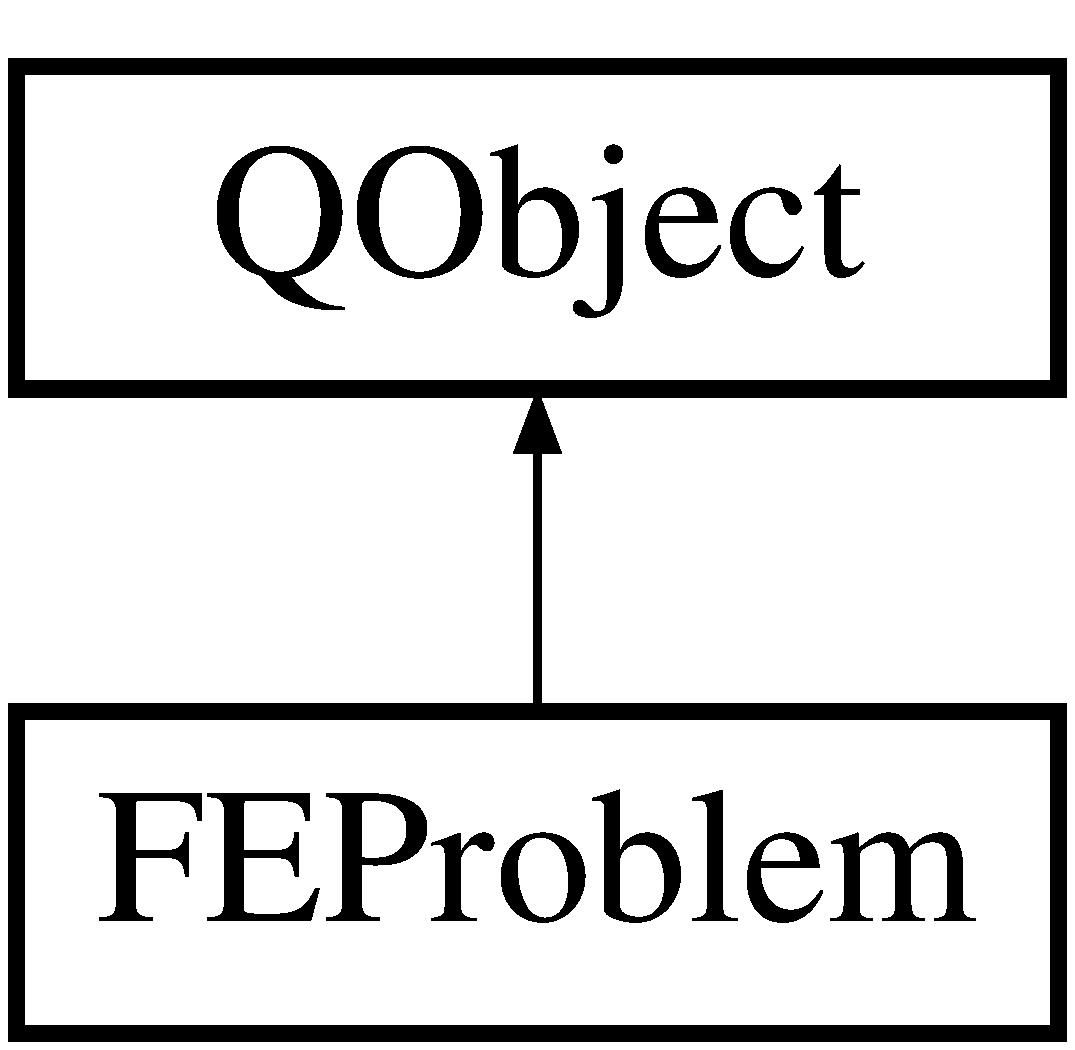
\includegraphics[height=2.000000cm]{class_f_e_problem}
\end{center}
\end{figure}
\subsection*{Public Slots}
\begin{DoxyCompactItemize}
\item 
void {\bfseries Process\+Param\+Data} ()\hypertarget{class_f_e_problem_a39624db202a3e8eb5de7e23312852c03}{}\label{class_f_e_problem_a39624db202a3e8eb5de7e23312852c03}

\end{DoxyCompactItemize}
\subsection*{Public Member Functions}
\begin{DoxyCompactItemize}
\item 
{\bfseries F\+E\+Problem} (\hyperlink{class_maillage3_d}{Maillage3D} $\ast$\+\_\+maillage, \hyperlink{class_r_h_s}{R\+HS} $\ast$\+\_\+rhs, \hyperlink{class_b_c}{BC} $\ast$\+\_\+bc, int \+\_\+op, bool \+\_\+unit)\hypertarget{class_f_e_problem_a2533222abf90fc2d04a4234a1014f297}{}\label{class_f_e_problem_a2533222abf90fc2d04a4234a1014f297}

\item 
void {\bfseries ClearA} ()\hypertarget{class_f_e_problem_a8cfe4ef4c62f979abddf7cbbf4eb865d}{}\label{class_f_e_problem_a8cfe4ef4c62f979abddf7cbbf4eb865d}

\item 
\hyperlink{class_c3}{C3} {\bfseries Calc\+Int\+On\+Triangle} (\hyperlink{class_maillage3_d}{Maillage3D} $\ast$\+\_\+maillage, \hyperlink{class_b_c}{BC} $\ast$\+\_\+bc, int idx, int tri\+\_\+idx)\hypertarget{class_f_e_problem_a0840b3f7f979205c10c6e0540fd351f3}{}\label{class_f_e_problem_a0840b3f7f979205c10c6e0540fd351f3}

\item 
\hyperlink{class_c3}{C3} {\bfseries Calc\+Int\+On\+Tetrahedron} (\hyperlink{class_maillage3_d}{Maillage3D} $\ast$\+\_\+maillage, \hyperlink{class_r_h_s}{R\+HS} $\ast$\+\_\+bc, int idx, int tetra\+\_\+idx)\hypertarget{class_f_e_problem_a488637fda62991b5f6e41ce6b6c67234}{}\label{class_f_e_problem_a488637fda62991b5f6e41ce6b6c67234}

\item 
void {\bfseries Build\+Poisson\+Operator} ()\hypertarget{class_f_e_problem_a93b43c73b15cd0fc2e794f8c9a95c3b4}{}\label{class_f_e_problem_a93b43c73b15cd0fc2e794f8c9a95c3b4}

\item 
void {\bfseries Build\+Parameter\+Poisson\+Operator} (double lambda)\hypertarget{class_f_e_problem_a88a0511cfde10f33442b0f31f0f4840e}{}\label{class_f_e_problem_a88a0511cfde10f33442b0f31f0f4840e}

\item 
void {\bfseries Build\+Partitionned\+Parameter\+Poisson\+Operator} (std\+::map$<$ int, double $>$ lambdas, std\+::map$<$ int, int $>$ $\ast$partition\+\_\+data)\hypertarget{class_f_e_problem_ae7f707511e3f03879a4c37de25af262f}{}\label{class_f_e_problem_ae7f707511e3f03879a4c37de25af262f}

\item 
void {\bfseries Build\+Heat\+Operator} ()\hypertarget{class_f_e_problem_a28324e797fb63c2eb6f1290961707c5c}{}\label{class_f_e_problem_a28324e797fb63c2eb6f1290961707c5c}

\item 
void {\bfseries Build\+Parameter\+Heat\+Operator} (double lambda)\hypertarget{class_f_e_problem_a7e5f1a4a65eb0d6aed9dbabf92bc0da8}{}\label{class_f_e_problem_a7e5f1a4a65eb0d6aed9dbabf92bc0da8}

\item 
void {\bfseries Build\+Partitionned\+Parameter\+Heat\+Operator} (std\+::map$<$ int, double $>$ lambdas, std\+::map$<$ int, int $>$ $\ast$partition\+\_\+data)\hypertarget{class_f_e_problem_a8f31694c860f6c4328435a03ba49a16f}{}\label{class_f_e_problem_a8f31694c860f6c4328435a03ba49a16f}

\item 
void {\bfseries Build\+Helmholtz\+Operator} ()\hypertarget{class_f_e_problem_abf351263b822451ef3a9e426c5a24fb3}{}\label{class_f_e_problem_abf351263b822451ef3a9e426c5a24fb3}

\item 
void {\bfseries Build\+Parameter\+Helmholtz\+Operator} (double omega)\hypertarget{class_f_e_problem_a47be6792b07ddfe598e9baab37b5d442}{}\label{class_f_e_problem_a47be6792b07ddfe598e9baab37b5d442}

\item 
void {\bfseries Build\+Partitionned\+Parameter\+Helmholtz\+Operator} (std\+::map$<$ int, double $>$ omegas, std\+::map$<$ int, int $>$ $\ast$partition\+\_\+data)\hypertarget{class_f_e_problem_a666ceb9dd40eb18d8f825e81a4946b96}{}\label{class_f_e_problem_a666ceb9dd40eb18d8f825e81a4946b96}

\item 
void {\bfseries Display\+Elementary\+Mass\+Matrix} (int n\+\_\+elem)\hypertarget{class_f_e_problem_a84a7d802bed7528c88c34ec7d7d9c243}{}\label{class_f_e_problem_a84a7d802bed7528c88c34ec7d7d9c243}

\item 
void {\bfseries Display\+Elementary\+Stiffness\+Matrix} (int n\+\_\+elem)\hypertarget{class_f_e_problem_a2c7f81c3c19f2084786c05fa62bb2a16}{}\label{class_f_e_problem_a2c7f81c3c19f2084786c05fa62bb2a16}

\item 
\hyperlink{class_vector_c3}{Vector\+C3} {\bfseries Get\+BC} ()\hypertarget{class_f_e_problem_ae35d33f28900ab65cfda40dadbc37032}{}\label{class_f_e_problem_ae35d33f28900ab65cfda40dadbc37032}

\item 
\hyperlink{class_vector_c3}{Vector\+C3} {\bfseries Get\+R\+HS} ()\hypertarget{class_f_e_problem_a8430129189603424a40ed0d5fe532cce}{}\label{class_f_e_problem_a8430129189603424a40ed0d5fe532cce}

\item 
\hyperlink{class_mat_sparse_c3}{Mat\+Sparse\+C3} $\ast$ {\bfseries GetA} ()\hypertarget{class_f_e_problem_ab8d3a04c8c349cc5071b2f2e234b9f89}{}\label{class_f_e_problem_ab8d3a04c8c349cc5071b2f2e234b9f89}

\end{DoxyCompactItemize}


The documentation for this class was generated from the following files\+:\begin{DoxyCompactItemize}
\item 
E\+F-\/\+Solver/feproblem.\+h\item 
E\+F-\/\+Solver/feproblem.\+cpp\end{DoxyCompactItemize}

\hypertarget{class_maillage3_d}{}\section{Maillage3D Class Reference}
\label{class_maillage3_d}\index{Maillage3D@{Maillage3D}}
\subsection*{Public Member Functions}
\begin{DoxyCompactItemize}
\item 
{\bfseries Maillage3D} (ifstream \&file)\hypertarget{class_maillage3_d_a4cb644d6eb850e43cedbf76d6a0c7670}{}\label{class_maillage3_d_a4cb644d6eb850e43cedbf76d6a0c7670}

\item 
vector$<$ int $>$ $\ast$ {\bfseries Get\+Partitions\+Map} ()\hypertarget{class_maillage3_d_a67233581efb7b8c3871e6e790c194ad0}{}\label{class_maillage3_d_a67233581efb7b8c3871e6e790c194ad0}

\item 
map$<$ int, int $>$ $\ast$ {\bfseries Get\+Partition\+Data\+Map} ()\hypertarget{class_maillage3_d_a39d95905ed37c2648c823a8b1cf49201}{}\label{class_maillage3_d_a39d95905ed37c2648c823a8b1cf49201}

\item 
map$<$ int, \hyperlink{class_r3}{R3} $>$ $\ast$ {\bfseries Get\+Nodes\+Map} ()\hypertarget{class_maillage3_d_ac9fb51e0a9321c7517c034933fa7784b}{}\label{class_maillage3_d_ac9fb51e0a9321c7517c034933fa7784b}

\item 
map$<$ int, \hyperlink{class_r3}{R3} $>$ $\ast$ {\bfseries Get\+Boundary\+Nodes\+Map} ()\hypertarget{class_maillage3_d_a0d2839624de6ccc1c875a9ead1877dfc}{}\label{class_maillage3_d_a0d2839624de6ccc1c875a9ead1877dfc}

\item 
map$<$ int, tuple$<$ int, int, int, int $>$ $>$ $\ast$ {\bfseries Get\+Elements\+Map} ()\hypertarget{class_maillage3_d_a1b6ae9e950380f2b7e8fae2b229779e6}{}\label{class_maillage3_d_a1b6ae9e950380f2b7e8fae2b229779e6}

\item 
map$<$ int, set$<$ int $>$ $\ast$ $>$ $\ast$ {\bfseries Get\+Neighbours\+Map} ()\hypertarget{class_maillage3_d_aa2adbe2eacaa1fc937bc649c044a6ce3}{}\label{class_maillage3_d_aa2adbe2eacaa1fc937bc649c044a6ce3}

\item 
map$<$ int, set$<$ int $>$ $\ast$ $>$ $\ast$ {\bfseries Get\+Neighbours\+Elements\+Map} ()\hypertarget{class_maillage3_d_a9128a84b0d0490426f1686625cc1b96e}{}\label{class_maillage3_d_a9128a84b0d0490426f1686625cc1b96e}

\item 
map$<$ int, set$<$ int $>$ $\ast$ $>$ $\ast$ {\bfseries Get\+Neighbours\+Faces\+Map} ()\hypertarget{class_maillage3_d_a66c77483c54d224a33d18f94a6358c21}{}\label{class_maillage3_d_a66c77483c54d224a33d18f94a6358c21}

\item 
map$<$ int, tuple$<$ int, int, int $>$ $>$ $\ast$ {\bfseries Get\+Faces\+Map} ()\hypertarget{class_maillage3_d_ad025d923936e118f28f58da6678b68a5}{}\label{class_maillage3_d_ad025d923936e118f28f58da6678b68a5}

\item 
map$<$ int, tuple$<$ int, int, int $>$ $>$ $\ast$ {\bfseries Get\+Boundary\+Faces\+Map} ()\hypertarget{class_maillage3_d_a17c2008e3ce49edbb663b4e94a128a5e}{}\label{class_maillage3_d_a17c2008e3ce49edbb663b4e94a128a5e}

\item 
map$<$ int, pair$<$ int, int $>$ $>$ $\ast$ {\bfseries Get\+Triangles\+Interface\+Map} ()\hypertarget{class_maillage3_d_a8579c71a9e0416421a82ea67c5cf2adb}{}\label{class_maillage3_d_a8579c71a9e0416421a82ea67c5cf2adb}

\item 
map$<$ int, tuple$<$ int, int, int $>$ $>$ $\ast$ {\bfseries Get\+Triangles\+Nodes\+Interface\+Map} ()\hypertarget{class_maillage3_d_a48acf283b9bebf3c1c618a7337f279e1}{}\label{class_maillage3_d_a48acf283b9bebf3c1c618a7337f279e1}

\item 
int {\bfseries Get\+Partition\+Size} (int part)\hypertarget{class_maillage3_d_a345cbc564a1653bead5a2508b1b1b132}{}\label{class_maillage3_d_a345cbc564a1653bead5a2508b1b1b132}

\item 
int {\bfseries Get\+Elements\+Size} ()\hypertarget{class_maillage3_d_a0e71069f7b043621238c72167ef1fa2b}{}\label{class_maillage3_d_a0e71069f7b043621238c72167ef1fa2b}

\item 
int {\bfseries Get\+Faces\+Size} ()\hypertarget{class_maillage3_d_aa901d66f5755580392f62a38531552fe}{}\label{class_maillage3_d_aa901d66f5755580392f62a38531552fe}

\item 
int {\bfseries Get\+Edges\+Size} ()\hypertarget{class_maillage3_d_a1fc61fb4772dc1351615be462ef9c057}{}\label{class_maillage3_d_a1fc61fb4772dc1351615be462ef9c057}

\item 
int {\bfseries Get\+Nodes\+Size} ()\hypertarget{class_maillage3_d_a3e4211e571e2bfeb5b71527b1eb90f9f}{}\label{class_maillage3_d_a3e4211e571e2bfeb5b71527b1eb90f9f}

\item 
map$<$ int, tuple$<$ int, int, int, int $>$ $>$\+::iterator {\bfseries Get\+Elements\+Begin\+Iterator} ()\hypertarget{class_maillage3_d_ac2efb256ab107604d7b38b274079e6cf}{}\label{class_maillage3_d_ac2efb256ab107604d7b38b274079e6cf}

\item 
map$<$ int, tuple$<$ int, int, int, int $>$ $>$\+::iterator {\bfseries Get\+Elements\+End\+Iterator} ()\hypertarget{class_maillage3_d_a9fd0670340a755340e0fd98f3974e327}{}\label{class_maillage3_d_a9fd0670340a755340e0fd98f3974e327}

\item 
int {\bfseries Get\+Elements\+First\+Node\+Index} (int tetr)\hypertarget{class_maillage3_d_a38e38c0780b249912ce4306af86475fc}{}\label{class_maillage3_d_a38e38c0780b249912ce4306af86475fc}

\item 
int {\bfseries Get\+Elements\+Second\+Node\+Index} (int tetr)\hypertarget{class_maillage3_d_ae4471b28638125300989caf8ba541391}{}\label{class_maillage3_d_ae4471b28638125300989caf8ba541391}

\item 
int {\bfseries Get\+Elements\+Third\+Node\+Index} (int tetr)\hypertarget{class_maillage3_d_ab848af39c137fc2c19c51f15066488ea}{}\label{class_maillage3_d_ab848af39c137fc2c19c51f15066488ea}

\item 
int {\bfseries Get\+Elements\+Fourth\+Node\+Index} (int tetr)\hypertarget{class_maillage3_d_a638a2fc7195de3bda56446146f4277d4}{}\label{class_maillage3_d_a638a2fc7195de3bda56446146f4277d4}

\item 
void {\bfseries Display\+Interfaces\+Elements} ()\hypertarget{class_maillage3_d_a909cf720c7d174a415b972cf528dac7f}{}\label{class_maillage3_d_a909cf720c7d174a415b972cf528dac7f}

\item 
void {\bfseries Display\+Interfaces\+Triangles} ()\hypertarget{class_maillage3_d_afc15ae92a1b7bd5193379b0d8897ac82}{}\label{class_maillage3_d_afc15ae92a1b7bd5193379b0d8897ac82}

\item 
void {\bfseries Display\+Boundary\+Elements} ()\hypertarget{class_maillage3_d_ad06d861b9da1be8b3b25fe291e507c49}{}\label{class_maillage3_d_ad06d861b9da1be8b3b25fe291e507c49}

\item 
void {\bfseries Display\+Basic\+Data} ()\hypertarget{class_maillage3_d_ac75a9dc094220de48de7019c7c26ed2e}{}\label{class_maillage3_d_ac75a9dc094220de48de7019c7c26ed2e}

\item 
void {\bfseries Create\+Interface\+Triangles} ()\hypertarget{class_maillage3_d_ad9f418d68538572cbac972ed06292ceb}{}\label{class_maillage3_d_ad9f418d68538572cbac972ed06292ceb}

\item 
int {\bfseries Export\+Mesh\+As\+O\+B\+J\+File} (string File\+Path, bool verbose=0)\hypertarget{class_maillage3_d_a83c7b21c6f33946ceb59fade2dbb93b5}{}\label{class_maillage3_d_a83c7b21c6f33946ceb59fade2dbb93b5}

\item 
pair$<$ bool, tuple$<$ int, int, int $>$ $>$ {\bfseries Common\+Triangle} (tuple$<$ int, int, int, int $>$, tuple$<$ int, int, int, int $>$)\hypertarget{class_maillage3_d_ad962a76ff2824457bb8dd0cfd19e0341}{}\label{class_maillage3_d_ad962a76ff2824457bb8dd0cfd19e0341}

\end{DoxyCompactItemize}


The documentation for this class was generated from the following files\+:\begin{DoxyCompactItemize}
\item 
E\+F-\/\+Solver/maillage3d.\+h\item 
E\+F-\/\+Solver/maillage3d.\+cpp\end{DoxyCompactItemize}

\hypertarget{class_m_a_p___main_window}{}\section{M\+A\+P\+\_\+\+Main\+Window Class Reference}
\label{class_m_a_p___main_window}\index{M\+A\+P\+\_\+\+Main\+Window@{M\+A\+P\+\_\+\+Main\+Window}}
Inheritance diagram for M\+A\+P\+\_\+\+Main\+Window\+:\begin{figure}[H]
\begin{center}
\leavevmode
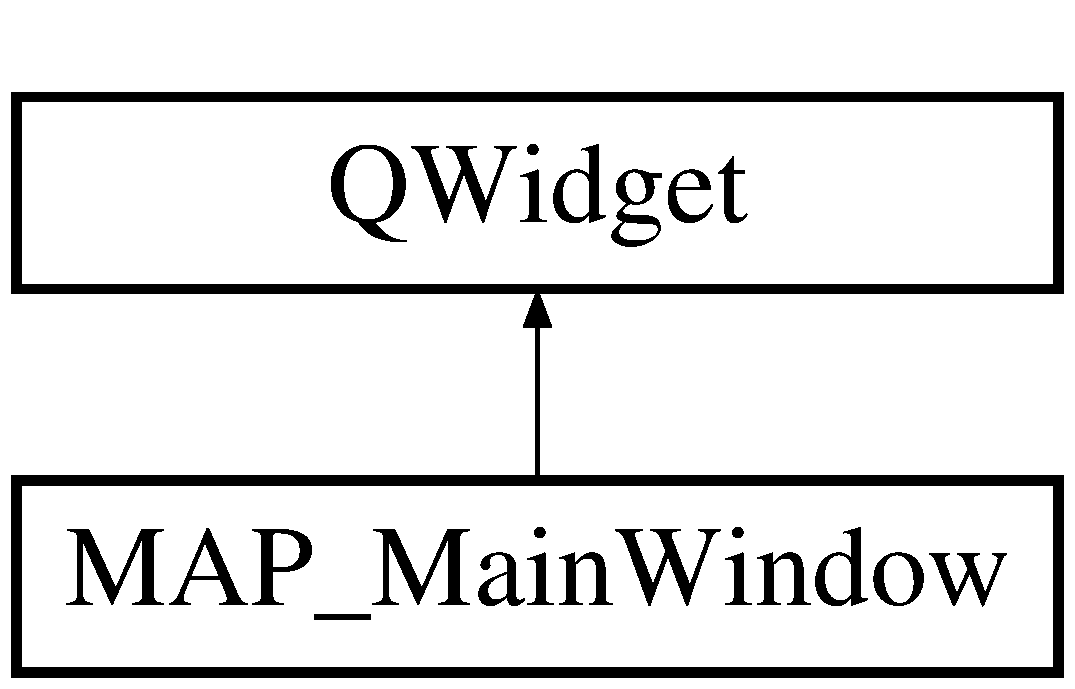
\includegraphics[height=2.000000cm]{class_m_a_p___main_window}
\end{center}
\end{figure}
\subsection*{Public Slots}
\begin{DoxyCompactItemize}
\item 
void {\bfseries on\+\_\+push\+Button\+\_\+load\+\_\+3\+D\+\_\+clicked} ()\hypertarget{class_m_a_p___main_window_ae4a6167f8bf7cbf951bd46176db08db7}{}\label{class_m_a_p___main_window_ae4a6167f8bf7cbf951bd46176db08db7}

\item 
void {\bfseries on\+\_\+push\+Button\+\_\+load\+\_\+\+R\+H\+S\+\_\+clicked} ()\hypertarget{class_m_a_p___main_window_a8c70320cb0812e595be1e00b78313ef8}{}\label{class_m_a_p___main_window_a8c70320cb0812e595be1e00b78313ef8}

\item 
void {\bfseries on\+\_\+push\+Button\+\_\+mat\+\_\+assemb\+\_\+clicked} ()\hypertarget{class_m_a_p___main_window_a981ee2396aa714dc4f866c5b54de8fb4}{}\label{class_m_a_p___main_window_a981ee2396aa714dc4f866c5b54de8fb4}

\item 
void {\bfseries on\+\_\+push\+Button\+\_\+load\+\_\+\+B\+C\+\_\+clicked} ()\hypertarget{class_m_a_p___main_window_a9645521f9d25fb884e3224808aae22e7}{}\label{class_m_a_p___main_window_a9645521f9d25fb884e3224808aae22e7}

\item 
void {\bfseries on\+\_\+push\+Button\+\_\+solve\+\_\+clicked} ()\hypertarget{class_m_a_p___main_window_a724b9dd161e1335adf30e2241dcfc7ee}{}\label{class_m_a_p___main_window_a724b9dd161e1335adf30e2241dcfc7ee}

\item 
void {\bfseries on\+\_\+push\+Button\+\_\+load\+\_\+\+Mat\+\_\+clicked} ()\hypertarget{class_m_a_p___main_window_a51bc8feda793ed3638d6e4f6ade21da3}{}\label{class_m_a_p___main_window_a51bc8feda793ed3638d6e4f6ade21da3}

\item 
void {\bfseries on\+\_\+push\+Button\+\_\+save\+\_\+output\+\_\+clicked} ()\hypertarget{class_m_a_p___main_window_a39a15dc6c6445758e02ec682f25c95ba}{}\label{class_m_a_p___main_window_a39a15dc6c6445758e02ec682f25c95ba}

\item 
void {\bfseries on\+\_\+push\+Button\+\_\+vis\+\_\+3\+D\+\_\+clicked} ()\hypertarget{class_m_a_p___main_window_ae9a7a0b27b489061a3d6563b186b439d}{}\label{class_m_a_p___main_window_ae9a7a0b27b489061a3d6563b186b439d}

\end{DoxyCompactItemize}
\subsection*{Public Member Functions}
\begin{DoxyCompactItemize}
\item 
{\bfseries M\+A\+P\+\_\+\+Main\+Window} (Q\+Widget $\ast$parent=0)\hypertarget{class_m_a_p___main_window_a33eac925ce07cdca9c41e22dd53aac2c}{}\label{class_m_a_p___main_window_a33eac925ce07cdca9c41e22dd53aac2c}

\item 
void {\bfseries Create\+Mesh\+Buffer} ()\hypertarget{class_m_a_p___main_window_acf8211bf8c159896e9786bd7be76e588}{}\label{class_m_a_p___main_window_acf8211bf8c159896e9786bd7be76e588}

\item 
void {\bfseries Assemble\+All} ()\hypertarget{class_m_a_p___main_window_af8f8064e36ccf1dd7dac276d5cb58299}{}\label{class_m_a_p___main_window_af8f8064e36ccf1dd7dac276d5cb58299}

\end{DoxyCompactItemize}


The documentation for this class was generated from the following files\+:\begin{DoxyCompactItemize}
\item 
E\+F-\/\+Solver/map\+\_\+mainwindow.\+h\item 
E\+F-\/\+Solver/map\+\_\+mainwindow.\+cpp\end{DoxyCompactItemize}

\hypertarget{class_mat_sparse_c3}{}\section{Mat\+Sparse\+C3 Class Reference}
\label{class_mat_sparse_c3}\index{Mat\+Sparse\+C3@{Mat\+Sparse\+C3}}
\subsection*{Public Member Functions}
\begin{DoxyCompactItemize}
\item 
{\bfseries Mat\+Sparse\+C3} (ifstream \&file)\hypertarget{class_mat_sparse_c3_a131b4ed2176c4133c07bb767238202e6}{}\label{class_mat_sparse_c3_a131b4ed2176c4133c07bb767238202e6}

\item 
int {\bfseries Diag\+Mat\+Mul} (\hyperlink{class_vector_c3}{Mat\+Diag})\hypertarget{class_mat_sparse_c3_a52f2549b2752a08a5bb5708f29aee6d1}{}\label{class_mat_sparse_c3_a52f2549b2752a08a5bb5708f29aee6d1}

\item 
int {\bfseries Mat\+Diag\+Mul} (\hyperlink{class_vector_c3}{Mat\+Diag})\hypertarget{class_mat_sparse_c3_aa378fe6d56a701a296fee6fe1f08d166}{}\label{class_mat_sparse_c3_aa378fe6d56a701a296fee6fe1f08d166}

\item 
void {\bfseries Mat\+Vect\+Mul} (\hyperlink{class_vector_c3}{Vector\+C3} \&i, \hyperlink{class_vector_c3}{Vector\+C3} \&o, int \+\_\+comp=-\/1) const \hypertarget{class_mat_sparse_c3_a646d02bcf55b7ee5b1259a291642c693}{}\label{class_mat_sparse_c3_a646d02bcf55b7ee5b1259a291642c693}

\item 
int {\bfseries Edit\+Profile\+From\+Mesh} (\hyperlink{class_maillage3_d}{Maillage3D})\hypertarget{class_mat_sparse_c3_a0e741ecd0918fd2a5353990386193a76}{}\label{class_mat_sparse_c3_a0e741ecd0918fd2a5353990386193a76}

\item 
int {\bfseries Insert} (int, int)\hypertarget{class_mat_sparse_c3_a14945b3885074a27b516796d597aadc8}{}\label{class_mat_sparse_c3_a14945b3885074a27b516796d597aadc8}

\item 
int {\bfseries Idx\+Search} (int i, int j)\hypertarget{class_mat_sparse_c3_a2e66f2ad85fdb75e9504935443eb2c3c}{}\label{class_mat_sparse_c3_a2e66f2ad85fdb75e9504935443eb2c3c}

\item 
\hyperlink{class_vector_c3}{Vector\+C3} \& {\bfseries Get\+Data} ()\hypertarget{class_mat_sparse_c3_a9c947b688cde1bbf3a7daf3f28444b26}{}\label{class_mat_sparse_c3_a9c947b688cde1bbf3a7daf3f28444b26}

\item 
KN$<$ int $>$ \& {\bfseries GetJ} ()\hypertarget{class_mat_sparse_c3_a000904c956166268f7c6c73d06170147}{}\label{class_mat_sparse_c3_a000904c956166268f7c6c73d06170147}

\item 
KN$<$ int $>$ \& {\bfseries GetP} ()\hypertarget{class_mat_sparse_c3_a208b1602440283d8bbab251386170441}{}\label{class_mat_sparse_c3_a208b1602440283d8bbab251386170441}

\item 
int {\bfseries Get\+Size} ()\hypertarget{class_mat_sparse_c3_a78ca20fe17ca028b13d4d1113b532208}{}\label{class_mat_sparse_c3_a78ca20fe17ca028b13d4d1113b532208}

\item 
void {\bfseries Display\+To\+Output\+\_\+\+Scilab} ()\hypertarget{class_mat_sparse_c3_ac1cdc341b34e014fd7d953d86b4e3d49}{}\label{class_mat_sparse_c3_ac1cdc341b34e014fd7d953d86b4e3d49}

\end{DoxyCompactItemize}


The documentation for this class was generated from the following files\+:\begin{DoxyCompactItemize}
\item 
E\+F-\/\+Solver/Mat\+Sparse\+C3.\+h\item 
E\+F-\/\+Solver/Mat\+Sparse\+C3.\+cpp\end{DoxyCompactItemize}

\hypertarget{class_orbit_transform_controller}{}\section{Orbit\+Transform\+Controller Class Reference}
\label{class_orbit_transform_controller}\index{Orbit\+Transform\+Controller@{Orbit\+Transform\+Controller}}
Inheritance diagram for Orbit\+Transform\+Controller\+:\begin{figure}[H]
\begin{center}
\leavevmode
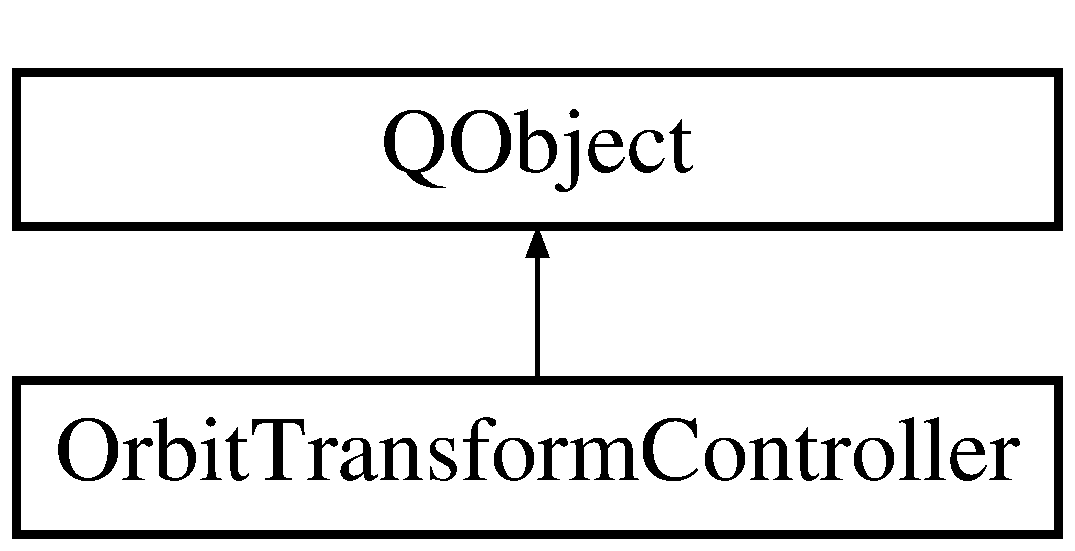
\includegraphics[height=2.000000cm]{class_orbit_transform_controller}
\end{center}
\end{figure}
\subsection*{Signals}
\begin{DoxyCompactItemize}
\item 
void {\bfseries target\+Changed} ()\hypertarget{class_orbit_transform_controller_af86371555346d6c85d0fada3f262a0cd}{}\label{class_orbit_transform_controller_af86371555346d6c85d0fada3f262a0cd}

\item 
void {\bfseries radius\+Changed} ()\hypertarget{class_orbit_transform_controller_a39ac6a5e8a31bb2ef1d4444baa95743e}{}\label{class_orbit_transform_controller_a39ac6a5e8a31bb2ef1d4444baa95743e}

\item 
void {\bfseries angle\+Changed} ()\hypertarget{class_orbit_transform_controller_acc3b82da234df20646e01721069c455e}{}\label{class_orbit_transform_controller_acc3b82da234df20646e01721069c455e}

\end{DoxyCompactItemize}
\subsection*{Public Member Functions}
\begin{DoxyCompactItemize}
\item 
{\bfseries Orbit\+Transform\+Controller} (Q\+Object $\ast$parent=0)\hypertarget{class_orbit_transform_controller_a45fa9bde3a0a7a1d57d879966a4056ac}{}\label{class_orbit_transform_controller_a45fa9bde3a0a7a1d57d879966a4056ac}

\item 
void {\bfseries set\+Target} (Qt3\+D\+Core\+::\+Q\+Transform $\ast$target)\hypertarget{class_orbit_transform_controller_a1a5651760f79cec5e5cac9e8a46411f7}{}\label{class_orbit_transform_controller_a1a5651760f79cec5e5cac9e8a46411f7}

\item 
Qt3\+D\+Core\+::\+Q\+Transform $\ast$ {\bfseries target} () const \hypertarget{class_orbit_transform_controller_a3cea976555311c54b8ae0b6ee22cce8e}{}\label{class_orbit_transform_controller_a3cea976555311c54b8ae0b6ee22cce8e}

\item 
void {\bfseries set\+Radius} (float radius)\hypertarget{class_orbit_transform_controller_aa39976e56c899dabc71ead7ec83df41a}{}\label{class_orbit_transform_controller_aa39976e56c899dabc71ead7ec83df41a}

\item 
float {\bfseries radius} () const \hypertarget{class_orbit_transform_controller_ac64ff74f6c8b5bbbce267e475bd44725}{}\label{class_orbit_transform_controller_ac64ff74f6c8b5bbbce267e475bd44725}

\item 
void {\bfseries set\+Angle} (float angle)\hypertarget{class_orbit_transform_controller_a3d59107dc7f63b535f477d65a4183303}{}\label{class_orbit_transform_controller_a3d59107dc7f63b535f477d65a4183303}

\item 
float {\bfseries angle} () const \hypertarget{class_orbit_transform_controller_aacb85bd74a4120fce4de237d84763017}{}\label{class_orbit_transform_controller_aacb85bd74a4120fce4de237d84763017}

\end{DoxyCompactItemize}
\subsection*{Protected Member Functions}
\begin{DoxyCompactItemize}
\item 
void {\bfseries update\+Matrix} ()\hypertarget{class_orbit_transform_controller_ad225ee6e4c6545a804d542606585f6dd}{}\label{class_orbit_transform_controller_ad225ee6e4c6545a804d542606585f6dd}

\end{DoxyCompactItemize}
\subsection*{Properties}
\begin{DoxyCompactItemize}
\item 
Qt3\+D\+Core\+::\+Q\+Transform {\bfseries target}\hypertarget{class_orbit_transform_controller_a1b887289a09be4ddef03f8f676f3b138}{}\label{class_orbit_transform_controller_a1b887289a09be4ddef03f8f676f3b138}

\item 
float {\bfseries radius}\hypertarget{class_orbit_transform_controller_a99c255042c9a78481954775edc7ec6e6}{}\label{class_orbit_transform_controller_a99c255042c9a78481954775edc7ec6e6}

\item 
float {\bfseries angle}\hypertarget{class_orbit_transform_controller_a923e23fca682a1012959b76a7f32cb10}{}\label{class_orbit_transform_controller_a923e23fca682a1012959b76a7f32cb10}

\end{DoxyCompactItemize}


The documentation for this class was generated from the following files\+:\begin{DoxyCompactItemize}
\item 
E\+F-\/\+Solver/orbittransformcontroller.\+h\item 
E\+F-\/\+Solver/orbittransformcontroller.\+cpp\end{DoxyCompactItemize}

\hypertarget{class_parameters_dialog}{}\section{Parameters\+Dialog Class Reference}
\label{class_parameters_dialog}\index{Parameters\+Dialog@{Parameters\+Dialog}}
Inheritance diagram for Parameters\+Dialog\+:\begin{figure}[H]
\begin{center}
\leavevmode
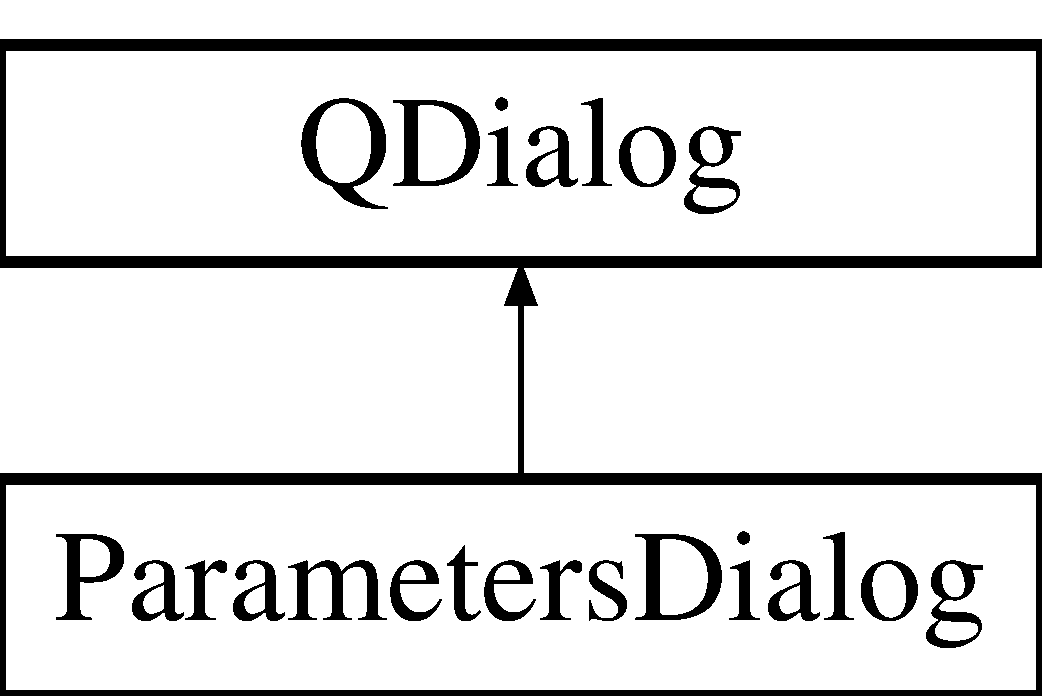
\includegraphics[height=2.000000cm]{class_parameters_dialog}
\end{center}
\end{figure}
\subsection*{Public Slots}
\begin{DoxyCompactItemize}
\item 
void {\bfseries on\+\_\+push\+Button\+\_\+validate\+\_\+released} ()\hypertarget{class_parameters_dialog_ae707e377abff2711184699b8535f31ba}{}\label{class_parameters_dialog_ae707e377abff2711184699b8535f31ba}

\item 
void {\bfseries on\+\_\+radio\+Button\+\_\+global\+\_\+toggled} ()\hypertarget{class_parameters_dialog_aade2d2d1938ddceb34f8e10808910582}{}\label{class_parameters_dialog_aade2d2d1938ddceb34f8e10808910582}

\end{DoxyCompactItemize}
\subsection*{Public Member Functions}
\begin{DoxyCompactItemize}
\item 
{\bfseries Parameters\+Dialog} (std\+::vector$<$ int $>$ $\ast$partitions, int \+\_\+op, Q\+Widget $\ast$parent=0)\hypertarget{class_parameters_dialog_a278b5296661943e82111b3cc4da63be1}{}\label{class_parameters_dialog_a278b5296661943e82111b3cc4da63be1}

\item 
Ui\+::\+Parameters\+Dialog $\ast$ {\bfseries Get\+UI} ()\hypertarget{class_parameters_dialog_a177971eb352e39591607ad9504f2c937}{}\label{class_parameters_dialog_a177971eb352e39591607ad9504f2c937}

\item 
std\+::map$<$ int, double $>$ {\bfseries Get\+Data} ()\hypertarget{class_parameters_dialog_a4eaf4d045178cf33a9a9cdeed657791f}{}\label{class_parameters_dialog_a4eaf4d045178cf33a9a9cdeed657791f}

\item 
int {\bfseries Get\+OP} ()\hypertarget{class_parameters_dialog_a4d0eed1465b66b3c06c5031744e3314f}{}\label{class_parameters_dialog_a4d0eed1465b66b3c06c5031744e3314f}

\end{DoxyCompactItemize}


The documentation for this class was generated from the following files\+:\begin{DoxyCompactItemize}
\item 
E\+F-\/\+Solver/parametersdialog.\+h\item 
E\+F-\/\+Solver/parametersdialog.\+cpp\end{DoxyCompactItemize}

\hypertarget{struct_point}{}\section{Point Struct Reference}
\label{struct_point}\index{Point@{Point}}
\subsection*{Public Member Functions}
\begin{DoxyCompactItemize}
\item 
{\bfseries Point} (float xp, float yp, float zp)\hypertarget{struct_point_a6e8f421360411c1c9d8d87a05a1f22d2}{}\label{struct_point_a6e8f421360411c1c9d8d87a05a1f22d2}

\item 
{\bfseries Point} (Q\+Vector3D pos, unsigned char r, unsigned char g, unsigned char b)\hypertarget{struct_point_adfb353e445b1d93e028e9c2d597f171d}{}\label{struct_point_adfb353e445b1d93e028e9c2d597f171d}

\end{DoxyCompactItemize}
\subsection*{Public Attributes}
\begin{DoxyCompactItemize}
\item 
Q\+Vector3D {\bfseries p}\hypertarget{struct_point_a9facf974a0d7e0c9ce3c642b8d72f247}{}\label{struct_point_a9facf974a0d7e0c9ce3c642b8d72f247}

\item 
Q\+Vector3D {\bfseries c}\hypertarget{struct_point_a61448de152eaac57b2eae5873fd9bf6e}{}\label{struct_point_a61448de152eaac57b2eae5873fd9bf6e}

\end{DoxyCompactItemize}


The documentation for this struct was generated from the following file\+:\begin{DoxyCompactItemize}
\item 
E\+F-\/\+Solver/utils.\+h\end{DoxyCompactItemize}

\hypertarget{class_qt3_d_widget}{}\section{Qt3\+D\+Widget Class Reference}
\label{class_qt3_d_widget}\index{Qt3\+D\+Widget@{Qt3\+D\+Widget}}
Inheritance diagram for Qt3\+D\+Widget\+:\begin{figure}[H]
\begin{center}
\leavevmode
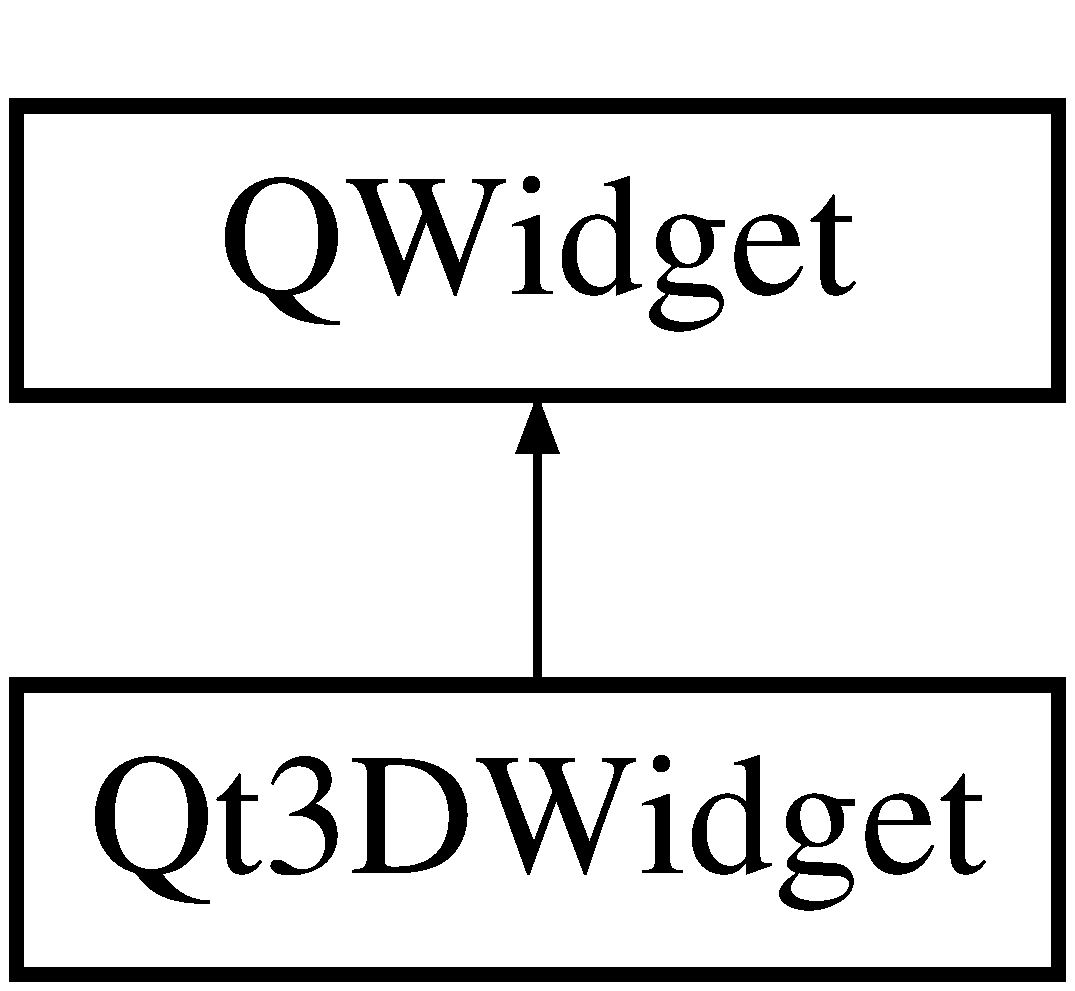
\includegraphics[height=2.000000cm]{class_qt3_d_widget}
\end{center}
\end{figure}
\subsection*{Public Member Functions}
\begin{DoxyCompactItemize}
\item 
{\bfseries Qt3\+D\+Widget} (Q\+Widget $\ast$parent=nullptr, std\+::vector$<$ \hyperlink{struct_triangle}{Triangle} $>$ $\ast$tris)\hypertarget{class_qt3_d_widget_a1effac984ac97784861c8f2eac331a8a}{}\label{class_qt3_d_widget_a1effac984ac97784861c8f2eac331a8a}

\end{DoxyCompactItemize}


The documentation for this class was generated from the following files\+:\begin{DoxyCompactItemize}
\item 
E\+F-\/\+Solver/qt3dwidget.\+h\item 
E\+F-\/\+Solver/qt3dwidget.\+cpp\end{DoxyCompactItemize}

\hypertarget{class_r2}{}\section{R2 Class Reference}
\label{class_r2}\index{R2@{R2}}
\subsection*{Public Member Functions}
\begin{DoxyCompactItemize}
\item 
{\bfseries R2} (R a, R b)\hypertarget{class_r2_a8d7d9af27c0e94323a3f775b71a0cfb6}{}\label{class_r2_a8d7d9af27c0e94323a3f775b71a0cfb6}

\item 
\hyperlink{class_r2}{R2} \& {\bfseries operator+=} (const \hyperlink{class_r2}{R2} \&P)\hypertarget{class_r2_ad7752be0cb083308920aeb8cd8eae2de}{}\label{class_r2_ad7752be0cb083308920aeb8cd8eae2de}

\item 
\hyperlink{class_r2}{R2} \& {\bfseries operator-\/=} (const \hyperlink{class_r2}{R2} \&P)\hypertarget{class_r2_addff4a2b70695ced44051ee1b5dbe360}{}\label{class_r2_addff4a2b70695ced44051ee1b5dbe360}

\item 
\hyperlink{class_r2}{R2} \& {\bfseries operator$\ast$=} (const R \&k)\hypertarget{class_r2_a14b5e1a68aaf96d8c4f19c7b0cf714b7}{}\label{class_r2_a14b5e1a68aaf96d8c4f19c7b0cf714b7}

\item 
\hyperlink{class_r2}{R2} \& {\bfseries operator/=} (const R \&k)\hypertarget{class_r2_a84ef02112ea25065158058cf97e28704}{}\label{class_r2_a84ef02112ea25065158058cf97e28704}

\item 
\hyperlink{class_r2}{R2} {\bfseries operator+} (\hyperlink{class_r2}{R2} \&P)\hypertarget{class_r2_aa07feaf6e1194c23c9b5fa31b3ad9976}{}\label{class_r2_aa07feaf6e1194c23c9b5fa31b3ad9976}

\item 
\hyperlink{class_r2}{R2} {\bfseries operator-\/} (\hyperlink{class_r2}{R2} \&P)\hypertarget{class_r2_ae9e490cc69cdf181bea7fcc393e84e5a}{}\label{class_r2_ae9e490cc69cdf181bea7fcc393e84e5a}

\item 
\hyperlink{class_r2}{R2} {\bfseries operator$\ast$} (R \&k)\hypertarget{class_r2_a4a4c6c822bd42536b506f959bc3d3fa3}{}\label{class_r2_a4a4c6c822bd42536b506f959bc3d3fa3}

\item 
\hyperlink{class_r2}{R2} {\bfseries operator/} (R \&k)\hypertarget{class_r2_af93a8e4a44d871d0330c647f56ab0d6f}{}\label{class_r2_af93a8e4a44d871d0330c647f56ab0d6f}

\item 
R {\bfseries operator,} (\hyperlink{class_r2}{R2} \&P)\hypertarget{class_r2_af741f4176f92a808b6d40d4c20af161f}{}\label{class_r2_af741f4176f92a808b6d40d4c20af161f}

\item 
\hyperlink{class_r2}{R2} {\bfseries operator+} () const \hypertarget{class_r2_a43ec9dd196c4c006ba2cf73c6c7317a3}{}\label{class_r2_a43ec9dd196c4c006ba2cf73c6c7317a3}

\item 
\hyperlink{class_r2}{R2} {\bfseries operator-\/} () const \hypertarget{class_r2_a6b64594c5483c1d56612efa3b52de65a}{}\label{class_r2_a6b64594c5483c1d56612efa3b52de65a}

\item 
R \& {\bfseries operator\mbox{[}$\,$\mbox{]}} (int i)\hypertarget{class_r2_a9648847349f8154bbdb3a0a86bb62ba2}{}\label{class_r2_a9648847349f8154bbdb3a0a86bb62ba2}

\item 
const R \& {\bfseries operator\mbox{[}$\,$\mbox{]}} (int i) const \hypertarget{class_r2_a457945edaa6b37c0aab2854208b61d87}{}\label{class_r2_a457945edaa6b37c0aab2854208b61d87}

\item 
R {\bfseries comp} (int i) const \hypertarget{class_r2_a6f99ccdcd33291ca61b38685a69565ca}{}\label{class_r2_a6f99ccdcd33291ca61b38685a69565ca}

\item 
R {\bfseries X\+\_\+} ()\hypertarget{class_r2_a31773713c895df08e2ee63e56dadb4e9}{}\label{class_r2_a31773713c895df08e2ee63e56dadb4e9}

\item 
R {\bfseries Y\+\_\+} ()\hypertarget{class_r2_a914b12a0f135ece9e36a8dbeeed71a46}{}\label{class_r2_a914b12a0f135ece9e36a8dbeeed71a46}

\end{DoxyCompactItemize}


The documentation for this class was generated from the following files\+:\begin{DoxyCompactItemize}
\item 
E\+F-\/\+Solver/R2.\+h\item 
E\+F-\/\+Solver/R2.\+cpp\end{DoxyCompactItemize}

\hypertarget{class_r3}{}\section{R3 Class Reference}
\label{class_r3}\index{R3@{R3}}
\subsection*{Public Member Functions}
\begin{DoxyCompactItemize}
\item 
{\bfseries R3} (R a, R b, R c)\hypertarget{class_r3_a37b08c627f9b80d28ef1b529d6c9393b}{}\label{class_r3_a37b08c627f9b80d28ef1b529d6c9393b}

\item 
\hyperlink{class_r3}{R3} \& {\bfseries operator+=} (const \hyperlink{class_r3}{R3} \&P)\hypertarget{class_r3_a7f8e93ee1556118d90955876f6680957}{}\label{class_r3_a7f8e93ee1556118d90955876f6680957}

\item 
\hyperlink{class_r3}{R3} \& {\bfseries operator-\/=} (const \hyperlink{class_r3}{R3} \&P)\hypertarget{class_r3_abb52da4099c6b0445da9328c734fca6d}{}\label{class_r3_abb52da4099c6b0445da9328c734fca6d}

\item 
\hyperlink{class_r3}{R3} \& {\bfseries operator$\ast$=} (const R \&k)\hypertarget{class_r3_af9c0985c2d02906c730bc704bda10c4d}{}\label{class_r3_af9c0985c2d02906c730bc704bda10c4d}

\item 
\hyperlink{class_r3}{R3} \& {\bfseries operator/=} (const R \&k)\hypertarget{class_r3_aec241319b6fb3190bbacabb54654b151}{}\label{class_r3_aec241319b6fb3190bbacabb54654b151}

\item 
bool {\bfseries operator==} (\hyperlink{class_r3}{R3} P) const \hypertarget{class_r3_a65a27d5d32de6e120671ac59a9cb9eaa}{}\label{class_r3_a65a27d5d32de6e120671ac59a9cb9eaa}

\item 
\hyperlink{class_r3}{R3} {\bfseries operator+} (const \hyperlink{class_r3}{R3} \&P)\hypertarget{class_r3_aff923bf7190c24b2b678addc5c8a71d7}{}\label{class_r3_aff923bf7190c24b2b678addc5c8a71d7}

\item 
\hyperlink{class_r3}{R3} {\bfseries operator-\/} (const \hyperlink{class_r3}{R3} \&P)\hypertarget{class_r3_aefd70a29754d71c1488a58500e7d0c07}{}\label{class_r3_aefd70a29754d71c1488a58500e7d0c07}

\item 
\hyperlink{class_r3}{R3} {\bfseries operator$\ast$} (const R \&k)\hypertarget{class_r3_a16f5cf27bd706e6f94e5ff3afbece807}{}\label{class_r3_a16f5cf27bd706e6f94e5ff3afbece807}

\item 
\hyperlink{class_r3}{R3} {\bfseries operator$\ast$} (const \hyperlink{class_r3}{R3} \&P)\hypertarget{class_r3_ac05cab8019656499f0cbf3e6f0a70930}{}\label{class_r3_ac05cab8019656499f0cbf3e6f0a70930}

\item 
\hyperlink{class_r3}{R3} {\bfseries operator/} (const R \&k)\hypertarget{class_r3_a7df4b80e63d9735b9ba0f2bc67cfbdbf}{}\label{class_r3_a7df4b80e63d9735b9ba0f2bc67cfbdbf}

\item 
\hyperlink{class_r3}{R3} {\bfseries operator/} (const \hyperlink{class_r3}{R3} \&P)\hypertarget{class_r3_a957265c55c2cc6aefed7124d033e54b5}{}\label{class_r3_a957265c55c2cc6aefed7124d033e54b5}

\item 
R {\bfseries operator,} (const \hyperlink{class_r3}{R3} \&P)\hypertarget{class_r3_aa7dc3e3333800472c9b30babf2fbae10}{}\label{class_r3_aa7dc3e3333800472c9b30babf2fbae10}

\item 
\hyperlink{class_r3}{R3} {\bfseries operator+} () const \hypertarget{class_r3_a981e1374173fc048bd33055397597176}{}\label{class_r3_a981e1374173fc048bd33055397597176}

\item 
\hyperlink{class_r3}{R3} {\bfseries operator-\/} () const \hypertarget{class_r3_ad59675eaeb404f95f04984f8ac1c0d0f}{}\label{class_r3_ad59675eaeb404f95f04984f8ac1c0d0f}

\item 
\hyperlink{class_r3}{R3} {\bfseries sqrt\+\_\+} () const \hypertarget{class_r3_a0fbe5b79974d436abc08b849b7a2b99a}{}\label{class_r3_a0fbe5b79974d436abc08b849b7a2b99a}

\item 
R \& {\bfseries operator\mbox{[}$\,$\mbox{]}} (int i)\hypertarget{class_r3_a13759fa191e3ce8023095e189ef6e0e7}{}\label{class_r3_a13759fa191e3ce8023095e189ef6e0e7}

\item 
const R \& {\bfseries operator\mbox{[}$\,$\mbox{]}} (int i) const \hypertarget{class_r3_a2266169539d6cdb0eeeed7f9bc1b98a6}{}\label{class_r3_a2266169539d6cdb0eeeed7f9bc1b98a6}

\item 
\hyperlink{class_r3}{R3} {\bfseries div\+\_\+} (const \hyperlink{class_r3}{R3} \&P) const \hypertarget{class_r3_a704360076265d7b4e7660c1e08593a90}{}\label{class_r3_a704360076265d7b4e7660c1e08593a90}

\item 
R {\bfseries comp} (int i) const \hypertarget{class_r3_afb8e0fa9d7028873d8669f5545d26bc4}{}\label{class_r3_afb8e0fa9d7028873d8669f5545d26bc4}

\item 
\hyperlink{class_r3}{R3} {\bfseries inv} () const \hypertarget{class_r3_a0a6c9ade1ee39ec0baf415e8db0cf556}{}\label{class_r3_a0a6c9ade1ee39ec0baf415e8db0cf556}

\item 
double {\bfseries norm} () const \hypertarget{class_r3_a12083e309481e4769e51db4bd772c925}{}\label{class_r3_a12083e309481e4769e51db4bd772c925}

\item 
R {\bfseries X\+\_\+} () const \hypertarget{class_r3_a699149de054f8654456d69866663ab78}{}\label{class_r3_a699149de054f8654456d69866663ab78}

\item 
R {\bfseries Y\+\_\+} () const \hypertarget{class_r3_a25acf0bc622d27eb6501613dee127b98}{}\label{class_r3_a25acf0bc622d27eb6501613dee127b98}

\item 
R {\bfseries Z\+\_\+} () const \hypertarget{class_r3_ac33c49227baec220003f7ae9d2100eac}{}\label{class_r3_ac33c49227baec220003f7ae9d2100eac}

\end{DoxyCompactItemize}


The documentation for this class was generated from the following files\+:\begin{DoxyCompactItemize}
\item 
E\+F-\/\+Solver/R3.\+h\item 
E\+F-\/\+Solver/R3.\+cpp\end{DoxyCompactItemize}

\hypertarget{class_r_h_s}{}\section{R\+HS Class Reference}
\label{class_r_h_s}\index{R\+HS@{R\+HS}}
\subsection*{Public Member Functions}
\begin{DoxyCompactItemize}
\item 
{\bfseries R\+HS} (ifstream \&file, map$<$ int, \hyperlink{class_r3}{R3} $>$ $\ast$node\+\_\+data)\hypertarget{class_r_h_s_a6ba0686af026bf64e4d5eedd0bc369ed}{}\label{class_r_h_s_a6ba0686af026bf64e4d5eedd0bc369ed}

\item 
string $\ast$ {\bfseries Get\+Expr} ()\hypertarget{class_r_h_s_afef333d9b6c0d45b467e4056697c8e7d}{}\label{class_r_h_s_afef333d9b6c0d45b467e4056697c8e7d}

\item 
vector$<$ \hyperlink{class_c3}{C3} $>$ $\ast$ {\bfseries Get\+R\+HS} ()\hypertarget{class_r_h_s_ab31764877ce436e254dad7d5288e1942}{}\label{class_r_h_s_ab31764877ce436e254dad7d5288e1942}

\item 
int {\bfseries Get\+Size} ()\hypertarget{class_r_h_s_a77b9a6902dd139acb20c5f5f8f05cd58}{}\label{class_r_h_s_a77b9a6902dd139acb20c5f5f8f05cd58}

\end{DoxyCompactItemize}


The documentation for this class was generated from the following files\+:\begin{DoxyCompactItemize}
\item 
E\+F-\/\+Solver/rhs.\+h\item 
E\+F-\/\+Solver/rhs.\+cpp\end{DoxyCompactItemize}

\hypertarget{class_scatter_data_modifier}{}\section{Scatter\+Data\+Modifier Class Reference}
\label{class_scatter_data_modifier}\index{Scatter\+Data\+Modifier@{Scatter\+Data\+Modifier}}
Inheritance diagram for Scatter\+Data\+Modifier\+:\begin{figure}[H]
\begin{center}
\leavevmode
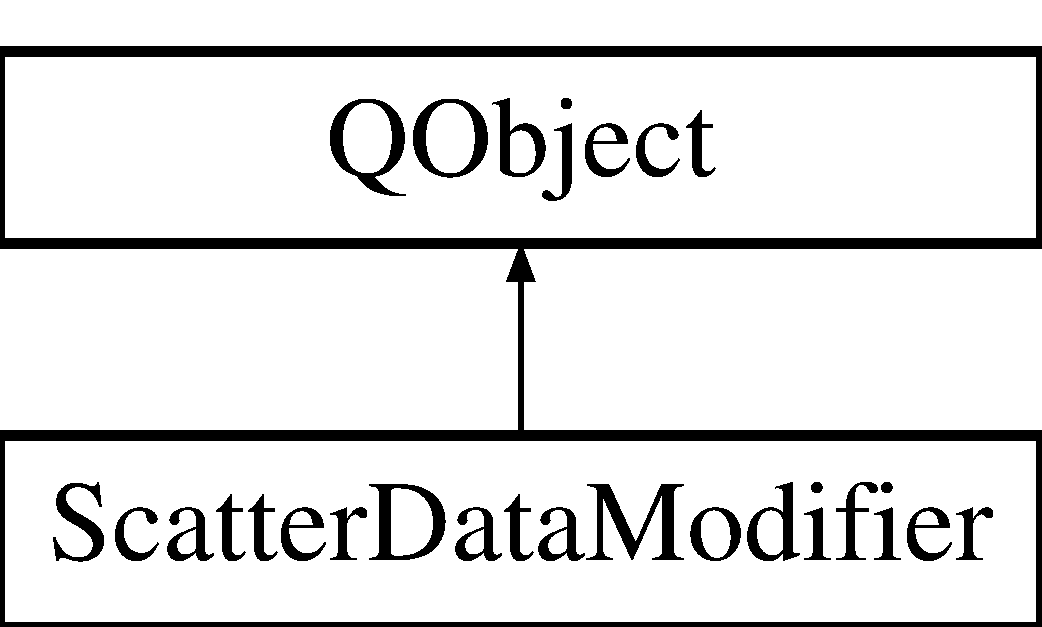
\includegraphics[height=2.000000cm]{class_scatter_data_modifier}
\end{center}
\end{figure}
\subsection*{Public Slots}
\begin{DoxyCompactItemize}
\item 
void {\bfseries change\+Style} (int style)\hypertarget{class_scatter_data_modifier_aa611530212bcdbecdd178a62fc4fc814}{}\label{class_scatter_data_modifier_aa611530212bcdbecdd178a62fc4fc814}

\item 
void {\bfseries change\+Theme} (int theme)\hypertarget{class_scatter_data_modifier_af99b708936c5f34af1ccb6c71b82642c}{}\label{class_scatter_data_modifier_af99b708936c5f34af1ccb6c71b82642c}

\item 
void {\bfseries change\+Shadow\+Quality} (int quality)\hypertarget{class_scatter_data_modifier_a2e160680fbbcea470a23f4c68e1d3207}{}\label{class_scatter_data_modifier_a2e160680fbbcea470a23f4c68e1d3207}

\item 
void {\bfseries shadow\+Quality\+Updated\+By\+Visual} (Q\+Abstract3\+D\+Graph\+::\+Shadow\+Quality shadow\+Quality)\hypertarget{class_scatter_data_modifier_a04be737d91afae1b3ae247b63a5de3a4}{}\label{class_scatter_data_modifier_a04be737d91afae1b3ae247b63a5de3a4}

\end{DoxyCompactItemize}
\subsection*{Signals}
\begin{DoxyCompactItemize}
\item 
void {\bfseries background\+Enabled\+Changed} (bool enabled)\hypertarget{class_scatter_data_modifier_ad95344ac8e42562517af82279348c146}{}\label{class_scatter_data_modifier_ad95344ac8e42562517af82279348c146}

\item 
void {\bfseries grid\+Enabled\+Changed} (bool enabled)\hypertarget{class_scatter_data_modifier_ae98a57da35a1354df2a4fd700cd2538a}{}\label{class_scatter_data_modifier_ae98a57da35a1354df2a4fd700cd2538a}

\item 
void {\bfseries shadow\+Quality\+Changed} (int quality)\hypertarget{class_scatter_data_modifier_adae4638a2e3c43a6fb16a788913a136c}{}\label{class_scatter_data_modifier_adae4638a2e3c43a6fb16a788913a136c}

\item 
void {\bfseries font\+Changed} (Q\+Font font)\hypertarget{class_scatter_data_modifier_aa0815d6660dc3e8530967220783abe87}{}\label{class_scatter_data_modifier_aa0815d6660dc3e8530967220783abe87}

\end{DoxyCompactItemize}
\subsection*{Public Member Functions}
\begin{DoxyCompactItemize}
\item 
{\bfseries Scatter\+Data\+Modifier} (Q3\+D\+Scatter $\ast$scatter, vector$<$ \hyperlink{struct_triangle}{Triangle} $>$ $\ast$mesh\+Vector, \hyperlink{class_vector_c3}{Vector\+C3} sol)\hypertarget{class_scatter_data_modifier_a09ad817005a3f86cc4e4505ede9a578b}{}\label{class_scatter_data_modifier_a09ad817005a3f86cc4e4505ede9a578b}

\item 
void {\bfseries add\+Data} ()\hypertarget{class_scatter_data_modifier_a5812ae3ac1e633b334c30dd717de9fe4}{}\label{class_scatter_data_modifier_a5812ae3ac1e633b334c30dd717de9fe4}

\item 
void {\bfseries change\+Style} ()\hypertarget{class_scatter_data_modifier_a9965097d382878cda8ea23be72582351}{}\label{class_scatter_data_modifier_a9965097d382878cda8ea23be72582351}

\item 
void {\bfseries change\+Preset\+Camera} ()\hypertarget{class_scatter_data_modifier_abf18c88b5e1c744f8fffb7179b748b75}{}\label{class_scatter_data_modifier_abf18c88b5e1c744f8fffb7179b748b75}

\item 
void {\bfseries change\+Label\+Style} ()\hypertarget{class_scatter_data_modifier_ad011038aa1c17d01603c2d01c383e7af}{}\label{class_scatter_data_modifier_ad011038aa1c17d01603c2d01c383e7af}

\item 
void {\bfseries change\+Font} (const Q\+Font \&font)\hypertarget{class_scatter_data_modifier_ab8afdc192cffb4a6332eef36cc83bc12}{}\label{class_scatter_data_modifier_ab8afdc192cffb4a6332eef36cc83bc12}

\item 
void {\bfseries change\+Font\+Size} (int fontsize)\hypertarget{class_scatter_data_modifier_ac9cc978e058c0d2e92aa39fa46748521}{}\label{class_scatter_data_modifier_ac9cc978e058c0d2e92aa39fa46748521}

\item 
void {\bfseries set\+Background\+Enabled} (int enabled)\hypertarget{class_scatter_data_modifier_a7ec5ec0558a9ec6b8dc924428bc9568a}{}\label{class_scatter_data_modifier_a7ec5ec0558a9ec6b8dc924428bc9568a}

\item 
void {\bfseries set\+Grid\+Enabled} (int enabled)\hypertarget{class_scatter_data_modifier_a8a0005f86ea76e5a3b2ae441978f4ff3}{}\label{class_scatter_data_modifier_a8a0005f86ea76e5a3b2ae441978f4ff3}

\item 
void {\bfseries set\+Smooth\+Dots} (int smooth)\hypertarget{class_scatter_data_modifier_aaa0369609bdb26c5c73a4bcee75a5bda}{}\label{class_scatter_data_modifier_aaa0369609bdb26c5c73a4bcee75a5bda}

\item 
void {\bfseries toggle\+Item\+Count} ()\hypertarget{class_scatter_data_modifier_a073aa3a6d52030a3b1b040ded1b80299}{}\label{class_scatter_data_modifier_a073aa3a6d52030a3b1b040ded1b80299}

\item 
void {\bfseries start} ()\hypertarget{class_scatter_data_modifier_ae1e22e1c27655905d3c7d9ac02517f5c}{}\label{class_scatter_data_modifier_ae1e22e1c27655905d3c7d9ac02517f5c}

\end{DoxyCompactItemize}


The documentation for this class was generated from the following files\+:\begin{DoxyCompactItemize}
\item 
E\+F-\/\+Solver/scatterdatamodifier.\+h\item 
E\+F-\/\+Solver/scatterdatamodifier.\+cpp\end{DoxyCompactItemize}

\hypertarget{class_scene_modifier}{}\section{Scene\+Modifier Class Reference}
\label{class_scene_modifier}\index{Scene\+Modifier@{Scene\+Modifier}}
Inheritance diagram for Scene\+Modifier\+:\begin{figure}[H]
\begin{center}
\leavevmode
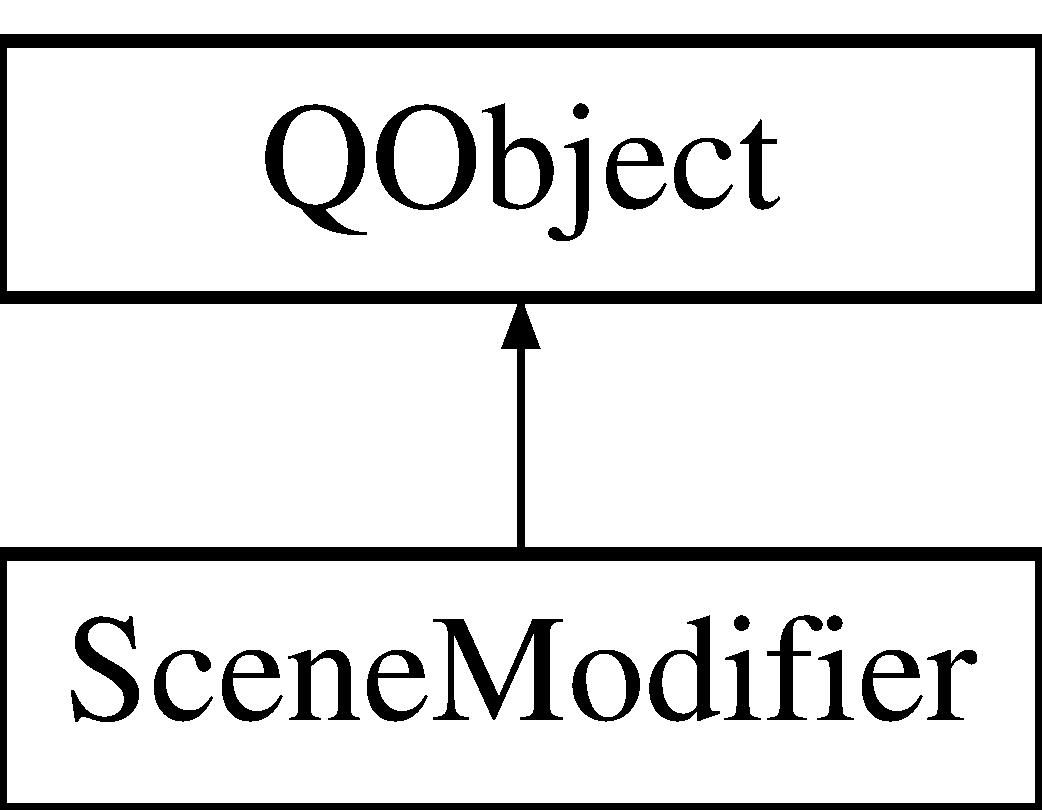
\includegraphics[height=2.000000cm]{class_scene_modifier}
\end{center}
\end{figure}
\subsection*{Public Member Functions}
\begin{DoxyCompactItemize}
\item 
{\bfseries Scene\+Modifier} (Qt3\+D\+Core\+::\+Q\+Entity $\ast$root\+Entity)\hypertarget{class_scene_modifier_acc07d34e62c8ff22c535f2b7f6478505}{}\label{class_scene_modifier_acc07d34e62c8ff22c535f2b7f6478505}

\item 
void {\bfseries add\+Triangle\+Mesh\+Custom\+Material} (Q\+String name, const std\+::vector$<$ \hyperlink{struct_triangle}{Triangle} $>$ $\ast$mesh\+Vector)\hypertarget{class_scene_modifier_a8fb7efb9da9f0cbd101c20ab3dc5f1a7}{}\label{class_scene_modifier_a8fb7efb9da9f0cbd101c20ab3dc5f1a7}

\end{DoxyCompactItemize}


The documentation for this class was generated from the following files\+:\begin{DoxyCompactItemize}
\item 
E\+F-\/\+Solver/scenemodifier.\+h\item 
E\+F-\/\+Solver/scenemodifier.\+cpp\end{DoxyCompactItemize}

\hypertarget{class_solver}{}\section{Solver Class Reference}
\label{class_solver}\index{Solver@{Solver}}
\subsection*{Public Member Functions}
\begin{DoxyCompactItemize}
\item 
{\bfseries Solver} (\hyperlink{class_f_e_problem}{F\+E\+Problem} $\ast$, Solver\+Method, double)\hypertarget{class_solver_aa2cf55d1dd4bc766e158333676d02907}{}\label{class_solver_aa2cf55d1dd4bc766e158333676d02907}

\item 
{\bfseries Solver} (\hyperlink{class_mat_sparse_c3}{Mat\+Sparse\+C3}, \hyperlink{class_vector_c3}{Vector\+C3}, Solver\+Method, double)\hypertarget{class_solver_a17df28f12239414a6ba9c69897d6495c}{}\label{class_solver_a17df28f12239414a6ba9c69897d6495c}

\item 
void {\bfseries init\+Solver} (int)\hypertarget{class_solver_a92e48ba76fe9154ab8270501488dd04d}{}\label{class_solver_a92e48ba76fe9154ab8270501488dd04d}

\item 
int {\bfseries Solve\+\_\+\+GC} ()\hypertarget{class_solver_a52310e223b4250a300690c703b74cc61}{}\label{class_solver_a52310e223b4250a300690c703b74cc61}

\item 
int {\bfseries Solve\+\_\+\+Orthodir} ()\hypertarget{class_solver_a0ae365806d42d59d6de9cfb6a2f5de24}{}\label{class_solver_a0ae365806d42d59d6de9cfb6a2f5de24}

\item 
int {\bfseries Solve\+\_\+\+G\+M\+R\+ES} ()\hypertarget{class_solver_a5ba090a92a672380ff0cb0902f138971}{}\label{class_solver_a5ba090a92a672380ff0cb0902f138971}

\item 
int {\bfseries Solve\+\_\+\+Min\+R\+ES} ()\hypertarget{class_solver_aa00ad25fcf01bdc9b10a94cead1ac433}{}\label{class_solver_aa00ad25fcf01bdc9b10a94cead1ac433}

\item 
\hyperlink{class_r3}{R3} {\bfseries compute\+Error} (Error\+Norm norm=Error\+Norm\+::infinity)\hypertarget{class_solver_a161542bed520dd70b7eaae65bff7c83f}{}\label{class_solver_a161542bed520dd70b7eaae65bff7c83f}

\item 
\hyperlink{class_r3}{R3} {\bfseries compute\+Error} (\hyperlink{class_mat_sparse_c3}{Mat\+Sparse\+C3} A, \hyperlink{class_vector_c3}{Vector\+C3} B, Error\+Norm norm=Error\+Norm\+::infinity)\hypertarget{class_solver_a87d7a1ec6b1dc58d6cf13031b25f6ff6}{}\label{class_solver_a87d7a1ec6b1dc58d6cf13031b25f6ff6}

\item 
void {\bfseries display\+Solution} ()\hypertarget{class_solver_a3f7ea5193c5e7f64deb6d6baf30d135c}{}\label{class_solver_a3f7ea5193c5e7f64deb6d6baf30d135c}

\item 
int {\bfseries Get\+Res} ()\hypertarget{class_solver_aeda9b18dda62b66d0d36467b7a1be89d}{}\label{class_solver_aeda9b18dda62b66d0d36467b7a1be89d}

\item 
\hyperlink{class_vector_c3}{Vector\+C3} {\bfseries Get\+Solution} ()\hypertarget{class_solver_a3f228651fbb74d274e8336285f79d14e}{}\label{class_solver_a3f228651fbb74d274e8336285f79d14e}

\end{DoxyCompactItemize}


The documentation for this class was generated from the following files\+:\begin{DoxyCompactItemize}
\item 
E\+F-\/\+Solver/solver.\+h\item 
E\+F-\/\+Solver/solver.\+cpp\end{DoxyCompactItemize}

\hypertarget{struct_triangle}{}\section{Triangle Struct Reference}
\label{struct_triangle}\index{Triangle@{Triangle}}
\subsection*{Public Member Functions}
\begin{DoxyCompactItemize}
\item 
{\bfseries Triangle} (\hyperlink{struct_point}{Point} p1, \hyperlink{struct_point}{Point} p2, \hyperlink{struct_point}{Point} p3)\hypertarget{struct_triangle_a690c761752314cccae3bfef93b27c511}{}\label{struct_triangle_a690c761752314cccae3bfef93b27c511}

\end{DoxyCompactItemize}
\subsection*{Public Attributes}
\begin{DoxyCompactItemize}
\item 
\hyperlink{struct_point}{Point} {\bfseries vertices} \mbox{[}3\mbox{]}\hypertarget{struct_triangle_a4a4048f6ca1c85dda63d64e509d479e0}{}\label{struct_triangle_a4a4048f6ca1c85dda63d64e509d479e0}

\end{DoxyCompactItemize}


The documentation for this struct was generated from the following file\+:\begin{DoxyCompactItemize}
\item 
E\+F-\/\+Solver/utils.\+h\end{DoxyCompactItemize}

\hypertarget{class_triangle_mesh_geometry}{}\section{Triangle\+Mesh\+Geometry Class Reference}
\label{class_triangle_mesh_geometry}\index{Triangle\+Mesh\+Geometry@{Triangle\+Mesh\+Geometry}}
Inheritance diagram for Triangle\+Mesh\+Geometry\+:\begin{figure}[H]
\begin{center}
\leavevmode
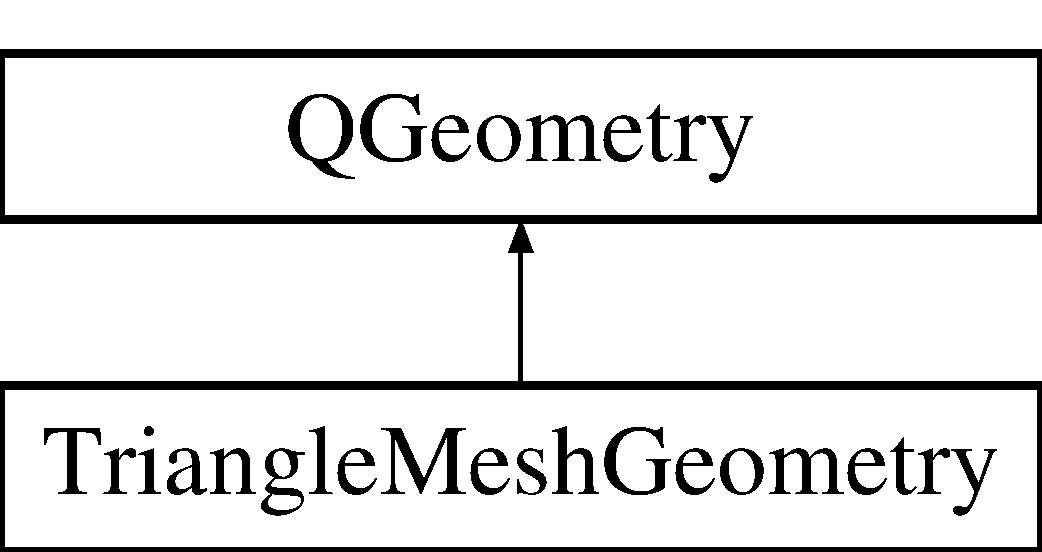
\includegraphics[height=2.000000cm]{class_triangle_mesh_geometry}
\end{center}
\end{figure}
\subsection*{Public Member Functions}
\begin{DoxyCompactItemize}
\item 
{\bfseries Triangle\+Mesh\+Geometry} (const std\+::vector$<$ \hyperlink{struct_triangle}{Triangle} $>$ $\ast$mesh\+Vector, \hyperlink{class_triangle_mesh_renderer}{Triangle\+Mesh\+Renderer} $\ast$parent)\hypertarget{class_triangle_mesh_geometry_a1957684e0853c59015cde9ee1cd05447}{}\label{class_triangle_mesh_geometry_a1957684e0853c59015cde9ee1cd05447}

\end{DoxyCompactItemize}


The documentation for this class was generated from the following files\+:\begin{DoxyCompactItemize}
\item 
E\+F-\/\+Solver/trianglemeshrenderer.\+h\item 
E\+F-\/\+Solver/trianglemeshrenderer.\+cpp\end{DoxyCompactItemize}

\hypertarget{class_triangle_mesh_renderer}{}\section{Triangle\+Mesh\+Renderer Class Reference}
\label{class_triangle_mesh_renderer}\index{Triangle\+Mesh\+Renderer@{Triangle\+Mesh\+Renderer}}
Inheritance diagram for Triangle\+Mesh\+Renderer\+:\begin{figure}[H]
\begin{center}
\leavevmode
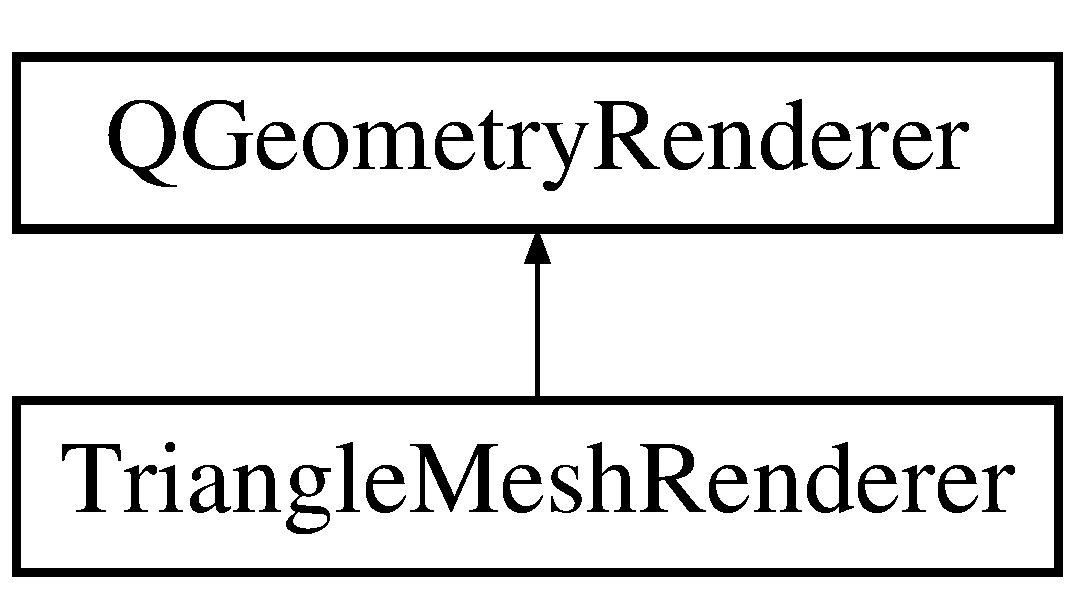
\includegraphics[height=2.000000cm]{class_triangle_mesh_renderer}
\end{center}
\end{figure}
\subsection*{Public Member Functions}
\begin{DoxyCompactItemize}
\item 
{\bfseries Triangle\+Mesh\+Renderer} (const std\+::vector$<$ \hyperlink{struct_triangle}{Triangle} $>$ $\ast$mesh\+Vector, Qt3\+D\+Core\+::\+Q\+Node $\ast$parent=0)\hypertarget{class_triangle_mesh_renderer_a1eb6d6afbd80596e0cc05a3b92dcb351}{}\label{class_triangle_mesh_renderer_a1eb6d6afbd80596e0cc05a3b92dcb351}

\end{DoxyCompactItemize}


The documentation for this class was generated from the following files\+:\begin{DoxyCompactItemize}
\item 
E\+F-\/\+Solver/trianglemeshrenderer.\+h\item 
E\+F-\/\+Solver/trianglemeshrenderer.\+cpp\end{DoxyCompactItemize}

\hypertarget{classutil}{}\section{util Class Reference}
\label{classutil}\index{util@{util}}
\subsection*{Static Public Member Functions}
\begin{DoxyCompactItemize}
\item 
static float {\bfseries eucl\+Distance} (\hyperlink{class_r2}{R2} \&a, \hyperlink{class_r2}{R2} \&b)\hypertarget{classutil_a3bc4c5cef5a34fa434f56f39d7e9c570}{}\label{classutil_a3bc4c5cef5a34fa434f56f39d7e9c570}

\item 
static float {\bfseries eucl\+Distance} (\hyperlink{class_r3}{R3} \&a, \hyperlink{class_r3}{R3} \&b)\hypertarget{classutil_a1a0dae5f5220e28dbfd2cd5cd18d067c}{}\label{classutil_a1a0dae5f5220e28dbfd2cd5cd18d067c}

\item 
static float {\bfseries scal\+Pdt} (\hyperlink{class_r2}{R2} \&a, \hyperlink{class_r2}{R2} \&b)\hypertarget{classutil_a3d34105fe5d136a536fcf17451544833}{}\label{classutil_a3d34105fe5d136a536fcf17451544833}

\item 
static float {\bfseries scal\+Pdt} (\hyperlink{class_r3}{R3} \&a, \hyperlink{class_r3}{R3} \&b)\hypertarget{classutil_a367fe70ffd37d85bde88eab2b8034c62}{}\label{classutil_a367fe70ffd37d85bde88eab2b8034c62}

\item 
static int {\bfseries type2nnodes} (int type)\hypertarget{classutil_a19c3bd928272e5450adeb2e33712b026}{}\label{classutil_a19c3bd928272e5450adeb2e33712b026}

\item 
static void {\bfseries print\+\_\+separator} ()\hypertarget{classutil_a12f34bfee4596aa886fbd8e32baad2c9}{}\label{classutil_a12f34bfee4596aa886fbd8e32baad2c9}

\item 
static int {\bfseries factorial} (int n)\hypertarget{classutil_a987089633ed64d5eb0c0a81e285a224f}{}\label{classutil_a987089633ed64d5eb0c0a81e285a224f}

\item 
static int {\bfseries kron} (int i, int j)\hypertarget{classutil_a69b0c210adb1707905053bd0e7155f87}{}\label{classutil_a69b0c210adb1707905053bd0e7155f87}

\item 
static double {\bfseries simplex3\+Mesure} (\hyperlink{class_r3}{R3} a, \hyperlink{class_r3}{R3} b, \hyperlink{class_r3}{R3} c, \hyperlink{class_r3}{R3} d)\hypertarget{classutil_a90f1098f73b1cef478c89d222f71a698}{}\label{classutil_a90f1098f73b1cef478c89d222f71a698}

\item 
static double {\bfseries simplex2\+Mesure} (\hyperlink{class_r3}{R3} a, \hyperlink{class_r3}{R3} b, \hyperlink{class_r3}{R3} c)\hypertarget{classutil_ae9613b3e4e2c8ad51148167c362804be}{}\label{classutil_ae9613b3e4e2c8ad51148167c362804be}

\end{DoxyCompactItemize}


The documentation for this class was generated from the following files\+:\begin{DoxyCompactItemize}
\item 
E\+F-\/\+Solver/utils.\+h\item 
E\+F-\/\+Solver/utils.\+cpp\end{DoxyCompactItemize}

\hypertarget{class_vector_c3}{}\section{Vector\+C3 Class Reference}
\label{class_vector_c3}\index{Vector\+C3@{Vector\+C3}}
\subsection*{Public Member Functions}
\begin{DoxyCompactItemize}
\item 
{\bfseries Vector\+C3} (KN$<$ C $>$ x, KN$<$ C $>$ y, KN$<$ C $>$ z)\hypertarget{class_vector_c3_a3819abec03018706500308e2fe760b47}{}\label{class_vector_c3_a3819abec03018706500308e2fe760b47}

\item 
{\bfseries Vector\+C3} (ifstream \&file)\hypertarget{class_vector_c3_aca464d063912b45a97fbf335e5fedb3a}{}\label{class_vector_c3_aca464d063912b45a97fbf335e5fedb3a}

\item 
int {\bfseries size} ()\hypertarget{class_vector_c3_a9d4a6d129dfce4a03433d81b686a78fe}{}\label{class_vector_c3_a9d4a6d129dfce4a03433d81b686a78fe}

\item 
void {\bfseries resize} (long nn)\hypertarget{class_vector_c3_a9dbc6aa027809d23fc8ecfd7e39a243e}{}\label{class_vector_c3_a9dbc6aa027809d23fc8ecfd7e39a243e}

\item 
void {\bfseries init} (long nn)\hypertarget{class_vector_c3_a5e04afad147dfb37c08f908a2c63ff95}{}\label{class_vector_c3_a5e04afad147dfb37c08f908a2c63ff95}

\item 
R {\bfseries Re\+\_\+norm} (int \+\_\+i=-\/1)\hypertarget{class_vector_c3_a11a75ef12bb63b654eef63d9d74fed17}{}\label{class_vector_c3_a11a75ef12bb63b654eef63d9d74fed17}

\item 
\hyperlink{class_c3}{C3} {\bfseries Re\+\_\+norms} ()    \hypertarget{class_vector_c3_ac1d57bba18095492caab53a4c91737da}{}\label{class_vector_c3_ac1d57bba18095492caab53a4c91737da}

\item 
\hyperlink{class_vector_c3}{Vector\+C3} \& {\bfseries operator+=} (\hyperlink{class_vector_c3}{Vector\+C3} P)\hypertarget{class_vector_c3_a02fea8573dea54a12d98175f944ae25d}{}\label{class_vector_c3_a02fea8573dea54a12d98175f944ae25d}

\item 
\hyperlink{class_vector_c3}{Vector\+C3} \& {\bfseries operator-\/=} (\hyperlink{class_vector_c3}{Vector\+C3} P)\hypertarget{class_vector_c3_a0d8f0d502e8a8a5eaff8dbdf8f3822b4}{}\label{class_vector_c3_a0d8f0d502e8a8a5eaff8dbdf8f3822b4}

\item 
\hyperlink{class_vector_c3}{Vector\+C3} \& {\bfseries operator$\ast$=} (const R k)\hypertarget{class_vector_c3_a7985367bd514306fe272bf6b5149fafc}{}\label{class_vector_c3_a7985367bd514306fe272bf6b5149fafc}

\item 
\hyperlink{class_vector_c3}{Vector\+C3} \& {\bfseries operator$\ast$=} (const C k)\hypertarget{class_vector_c3_ad560baf3374db280ea31bc6e705cf008}{}\label{class_vector_c3_ad560baf3374db280ea31bc6e705cf008}

\item 
\hyperlink{class_vector_c3}{Vector\+C3} \& {\bfseries operator$\ast$=} (\hyperlink{class_c3}{C3} k)\hypertarget{class_vector_c3_ae39fb73b248dfbc3031ec86b6c424d86}{}\label{class_vector_c3_ae39fb73b248dfbc3031ec86b6c424d86}

\item 
\hyperlink{class_vector_c3}{Vector\+C3} \& {\bfseries operator$\ast$=} (\hyperlink{class_r3}{R3} k)\hypertarget{class_vector_c3_a75bbde4e20d25a5894e63f604f8e3e3f}{}\label{class_vector_c3_a75bbde4e20d25a5894e63f604f8e3e3f}

\item 
\hyperlink{class_vector_c3}{Vector\+C3} \& {\bfseries operator/=} (const R k)\hypertarget{class_vector_c3_aa4e2f23e9702d378e75157f1ac0907c7}{}\label{class_vector_c3_aa4e2f23e9702d378e75157f1ac0907c7}

\item 
\hyperlink{class_vector_c3}{Vector\+C3} \& {\bfseries operator/=} (\hyperlink{class_r3}{R3} k)\hypertarget{class_vector_c3_a91cf16024658e17b75ea6dcc71a95fd6}{}\label{class_vector_c3_a91cf16024658e17b75ea6dcc71a95fd6}

\item 
\hyperlink{class_vector_c3}{Vector\+C3} \& {\bfseries operator/=} (\hyperlink{class_c3}{C3} k)\hypertarget{class_vector_c3_a692843a50f618b1a64d91c22248916e0}{}\label{class_vector_c3_a692843a50f618b1a64d91c22248916e0}

\item 
\hyperlink{class_vector_c3}{Vector\+C3} \& {\bfseries operator/=} (const C k)\hypertarget{class_vector_c3_adedb7160b722c14b7a006e3498287728}{}\label{class_vector_c3_adedb7160b722c14b7a006e3498287728}

\item 
void {\bfseries operator=} (\hyperlink{class_vector_c3}{Vector\+C3} P)\hypertarget{class_vector_c3_a8c133e29eb3733007be7ba0bbdadf190}{}\label{class_vector_c3_a8c133e29eb3733007be7ba0bbdadf190}

\item 
\hyperlink{class_vector_c3}{Vector\+C3} {\bfseries operator+} (\hyperlink{class_vector_c3}{Vector\+C3} P)\hypertarget{class_vector_c3_ae2765a2acbadf47e33502c619057b699}{}\label{class_vector_c3_ae2765a2acbadf47e33502c619057b699}

\item 
\hyperlink{class_vector_c3}{Vector\+C3} {\bfseries operator-\/} (\hyperlink{class_vector_c3}{Vector\+C3} P)\hypertarget{class_vector_c3_a9c03d0194fce8742b8bf92add8f0e3cc}{}\label{class_vector_c3_a9c03d0194fce8742b8bf92add8f0e3cc}

\item 
\hyperlink{class_vector_c3}{Vector\+C3} {\bfseries operator$\ast$} (C k)\hypertarget{class_vector_c3_a9365b497c814c95813bd8743f020b0f3}{}\label{class_vector_c3_a9365b497c814c95813bd8743f020b0f3}

\item 
\hyperlink{class_vector_c3}{Vector\+C3} {\bfseries operator$\ast$} (const \hyperlink{class_r3}{R3} \&k)\hypertarget{class_vector_c3_a1e1f6ebb846586a1e903bc61bfad408b}{}\label{class_vector_c3_a1e1f6ebb846586a1e903bc61bfad408b}

\item 
\hyperlink{class_vector_c3}{Vector\+C3} {\bfseries operator$\ast$} (const \hyperlink{class_c3}{C3} \&k)\hypertarget{class_vector_c3_adc374454d28460c1fa6de96da06a10fd}{}\label{class_vector_c3_adc374454d28460c1fa6de96da06a10fd}

\item 
\hyperlink{class_c3}{C3} {\bfseries operator,} (\hyperlink{class_vector_c3}{Vector\+C3} P)\hypertarget{class_vector_c3_ace99ee3f7501ff831cf1f47360b6bb08}{}\label{class_vector_c3_ace99ee3f7501ff831cf1f47360b6bb08}

\item 
void {\bfseries Display\+To\+Output\+\_\+\+Scilab} (int comp=0)\hypertarget{class_vector_c3_a0b5bba62609fd10699b9802f950ed452}{}\label{class_vector_c3_a0b5bba62609fd10699b9802f950ed452}

\end{DoxyCompactItemize}
\subsection*{Public Attributes}
\begin{DoxyCompactItemize}
\item 
KN$<$ C $>$ {\bfseries X} \mbox{[}3\mbox{]}\hypertarget{class_vector_c3_a9818588737fda61faa6bda68932294fc}{}\label{class_vector_c3_a9818588737fda61faa6bda68932294fc}

\end{DoxyCompactItemize}


The documentation for this class was generated from the following files\+:\begin{DoxyCompactItemize}
\item 
E\+F-\/\+Solver/Mat\+Sparse\+C3.\+h\item 
E\+F-\/\+Solver/Mat\+Sparse\+C3.\+cpp\end{DoxyCompactItemize}

\hypertarget{class_viewer3_d}{}\section{Viewer3D Class Reference}
\label{class_viewer3_d}\index{Viewer3D@{Viewer3D}}
Inheritance diagram for Viewer3D\+:\begin{figure}[H]
\begin{center}
\leavevmode
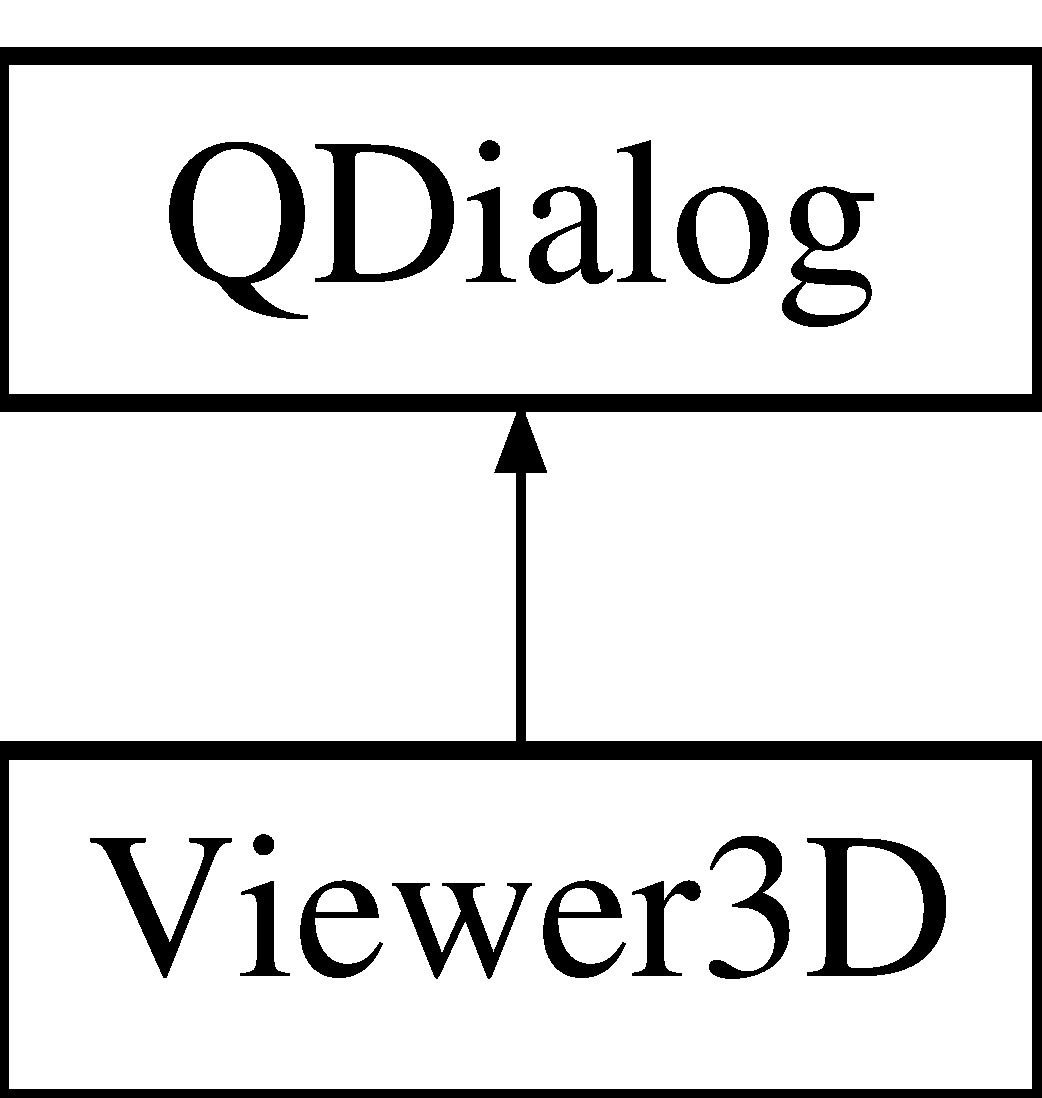
\includegraphics[height=2.000000cm]{class_viewer3_d}
\end{center}
\end{figure}
\subsection*{Public Member Functions}
\begin{DoxyCompactItemize}
\item 
{\bfseries Viewer3D} (Q\+Widget $\ast$parent=0)\hypertarget{class_viewer3_d_ae5635482d377cfd4f271803434de0dcf}{}\label{class_viewer3_d_ae5635482d377cfd4f271803434de0dcf}

\item 
\hyperlink{class_scene_modifier}{Scene\+Modifier} $\ast$ {\bfseries scene\+Modifier} ()\hypertarget{class_viewer3_d_af592d359d5e9b7b3f2f0c3ac005d1190}{}\label{class_viewer3_d_af592d359d5e9b7b3f2f0c3ac005d1190}

\end{DoxyCompactItemize}


The documentation for this class was generated from the following files\+:\begin{DoxyCompactItemize}
\item 
E\+F-\/\+Solver/viewer3d.\+h\item 
E\+F-\/\+Solver/viewer3d.\+cpp\end{DoxyCompactItemize}

\chapter{File Documentation}
\hypertarget{main_8cpp}{}\section{E\+F-\/\+Solver/main.cpp File Reference}
\label{main_8cpp}\index{E\+F-\/\+Solver/main.\+cpp@{E\+F-\/\+Solver/main.\+cpp}}


Programme de résolution de problèmes linéaire par la méthode des Elements Finis.  


{\ttfamily \#include \char`\"{}map\+\_\+mainwindow.\+h\char`\"{}}\\*
{\ttfamily \#include $<$Q\+Application$>$}\\*
{\ttfamily \#include \char`\"{}C3.\+h\char`\"{}}\\*
{\ttfamily \#include \char`\"{}utils.\+h\char`\"{}}\\*
\subsection*{Namespaces}
\begin{DoxyCompactItemize}
\item 
 \hyperlink{namespacestd}{std}
\begin{DoxyCompactList}\small\item\em Espace de nommage standard. \end{DoxyCompactList}\end{DoxyCompactItemize}
\subsection*{Functions}
\begin{DoxyCompactItemize}
\item 
int {\bfseries main} (int argc, char $\ast$argv\mbox{[}$\,$\mbox{]})\hypertarget{main_8cpp_a0ddf1224851353fc92bfbff6f499fa97}{}\label{main_8cpp_a0ddf1224851353fc92bfbff6f499fa97}

\end{DoxyCompactItemize}


\subsection{Detailed Description}
Programme de résolution de problèmes linéaire par la méthode des Elements Finis. 

\begin{DoxyAuthor}{Author}
Mehdi Ennaïme 
\end{DoxyAuthor}
\begin{DoxyVersion}{Version}
0.\+1 
\end{DoxyVersion}
\begin{DoxyDate}{Date}
20 Avril 2018
\end{DoxyDate}
Programme réalisant la résolution d\textquotesingle{}un problème d\textquotesingle{}E\+D\+Ps vectorielles linéaires par le biais de la méthode des élements finis 3D. Ce programme utilise des elements finis P1 
%--- End generated contents ---

% Index
\backmatter
\newpage
\phantomsection
\clearemptydoublepage
\addcontentsline{toc}{chapter}{Index}
\printindex

\end{document}
